\documentclass[master]{kuisthesis}
\jtitle{分数所有権に基づくメモリ解放安全性検証器}
\etitle{Static verifier for safe memory deallocation
based on fractional ownership}
\jauthor{大元 武}
\eauthor{Takeshi OMOTO}
\supervisor{末永 幸平}
\date{平成28年2月8日}
\department{通信情報システム}

\usepackage{amsmath, amssymb}
\usepackage{float}
\usepackage[dvipdfmx]{graphicx}
\usepackage{array}
\usepackage{ascmac}
\usepackage[marginpar]{todo}
\usepackage{url}
\usepackage{cite}
\usepackage{fancybox}
\usepackage{bcprules}
\usepackage{proof}
\usepackage{algorithm}
\usepackage{algpseudocode}
\usepackage{listings}
\usepackage{newtxtext}
%\usepackage{newtxmath}
%\usepackage{mathptmx}

%For listings
\lstset{
language={C},%
basicstyle=\ttfamily,%
commentstyle=\textit,%
classoffset=1,%
keywordstyle=\bfseries,%
frame=single,%
showstringspaces=false,%
numbers=left,
firstnumber=1,
stepnumber=1,
numberstyle=\footnotesize,%
captionpos=b,%
}%

\renewcommand{\lstlistingname}{Program}


\usepackage{theorem}

% For theorem
\theoremstyle{break}
\theorembodyfont{\normalfont}
\newtheorem{definition}{定義}
\newtheorem{theorem}{定理}
\newtheorem{example}{例}
\newtheorem{conjecture}{Conjecture}

% For algorithmic
% New definitions
\algnewcommand\algorithmicswitch{\textbf{switch}}
\algnewcommand\algorithmiccase{\textbf{case}:}
\algnewcommand\algorithmicdefault{\textbf{default}}
\algnewcommand\algorithmicassert{\texttt{assert}}
\algnewcommand\Assert[1]{\State \algorithmicassert(#1)}%
% New "environments"
\algdef{SE}[SWITCH]{Switch}{EndSwitch}[1]{\algorithmicswitch\ #1\ \algorithmicdo}{\algorithmicend\ \algorithmicswitch}%
\algdef{SE}[CASE]{Case}{EndCase}[1]{\algorithmiccase\ #1}{\algorithmicend\ \algorithmiccase}%
\algdef{SE}[DEFAULT]{Default}{EndDefault}[1]{\algorithmicdefault\ #1}{\algorithmicend\ \algorithmicdefault}%
\algtext*{EndSwitch}%
\algtext*{EndCase}%
\algtext*{EndDefault}%
% Renew definitions
\algrenewcommand\algorithmicfunction{\textbf{function}}
\algdef{SE}[FUNCTION]{Function}{EndFunction}[2]{\algorithmicfunction\ #1\ (#2)}{\algorithmicend\ \algorithmicfunction}%

%today
\newcounter{heisei}
\setcounter{heisei}{\number\year}
\addtocounter{heisei}{-1988}
\newcommand{\jtoday}{平成\theheisei 年\number\month 月\number\day 日}

%todo
\usepackage{xcolor}
\newcommand\mytodo[1]{\textcolor{red}{TODO:#1}}
\begin{document}
\maketitle
\begin{jabstract}
  C 言語では,プログラマは\verb|malloc|や\verb|free|などの命令を用いて,
  手動でメモリ管理を行わなければならない.そのため,メモリリークや,一度
  解放したメモリ領域へのアクセスなどの,メモリ管理上の誤りを起こすことが
  ある.

  SuenagaとKobayashiは,これらの誤りを静的に検出するための型システムを提
  案した.この型システムでは,ポインタを表す型を,\emph{所有権}と呼ばれる
  情報で拡張している.この情報は,プログラマがそのポインタを通してどのよ
  うな操作を行ってよいか,行わなければならないかを表している.プログラム
  に型がつけば,メモリ管理に関する誤りが起きないということが証明されてい
  る.彼らはこの型システムに基づいて,各変数や各関数にどのような型がつく
  のか自動で推論する型推論アルゴリズムを提案し,そのアルゴリズムに基づき
  検証器を実装した.型推論は,各命令から型付け規則に基づき,所有権が満た
  すべき制約式を生成し,その制約式の充足可能問題に帰着させている.

  しかし,彼らの型システムはC言語のサブセットを対象としているため,制御文
  など,いくつかの構文を扱うことができない.彼らの検証器は制御文も扱うこ
  とができるが,その部分の実装は厳密には理論に基づいたものにないっていな
  い.

  %彼らの検証器は,C 言語の全ての構文を扱うことができる.しかし,彼らの型
  %システムは,C言語のサブセットを対象としているため,制御文などいくつかの
  %構文は扱うことができない。そのため,彼らの検証器は,型推論アルゴリズム
  %に厳密に基づいたものになっていない。


  そこで本研究では,より信頼度の高い方法で検証器の実装を行う.具体的には,
  (1) 制御文で言語を拡張し,(2) その構文を扱えるように型システムを拡張す
  る.また,拡張した型システムに基づいて実装を行った.この検証器は,制御
  文に加えて,単方向リストなどのデータ構造や,相互再帰関数も扱うことがで
  きる.

  更に実装の利便性を高めるために\emph{型エラースライサー}を検証器に組み込
  んだ.型エラーが起こった場合,検証器は型エラーに関係する命令の行番号を
  表示する.この情報は,型エラーの原因を特定するのに役立つ.

  また,実装した検証器に対して予備実験を行った.検証器が制御文を含むプロ
  グラム,再帰のある構造体を扱ったプログラム,相互再帰関数を含むプログラ
  ムに対しても,メモリリークを正しく検出できることを確かめた.
\end{jabstract}
\begin{eabstract}

  Programming in the C language requires manual memory management using
  \verb|malloc| and \verb|free|.  Such memory management style is prone
  to bugs such as memory leak and an access to deallocated memory cells.

  Suenaga and Kobayashi proposed a type system for statically verifying
  memory-deallocation safety.  In this type system, a \emph {fractional
  ownership}, auxiliary information that expresses the capability and
  the obligation on a pointer, is assigned to each pointer type.  They
  proved that a well-typed program does not cause bugs related to memory
  deallocation.  They also proposed a type inference algorithm that
  automatically infers a type of each variable and each function and
  implemented a verifier based on the algorithm.  The type inference
  algorithm generates constraints that the ownerships should satisfy and
  checks the satisfiability of the constraints.

  However, their type system is designed only for a subset of the C
  language; it does not handle some statements such as control
  statements. Although their verifier supports the control statements,
  they support these statements in such a way that is not strictly based
  on the formally defined type inference algorithm.

  %Therefore, their verifier for C programs is not strictly based on the
  %formally defined type inference algorithm.

  %Their verifier can handle all statements of the C language.  However,
  %their type system is designed only for a subset of the C language
  %; it does not handle some statements of the C language such as control
  %statements. Therefore, their verifier for C programs is not strictly
  %based on the formally defined type inference algorithm.


  Our aim is to extend their framework so that it deals with the C
  language in a more dependable way.  Concretely, we extend (1) their
  language with the control statements and (2) the type system to handle
  these statements. We implement a verifier based on the extended type
  system.  Our implementation supports the control statements, data
  structures such as singly linked lists, and definitions of mutually
  recursive functions.

  In order to make the implementation more useful, we incorporate a
  \emph{type-error slicer} to our verifier.  If a program is not
  well-typed, the verifier displays the line numbers of the commands in
  the program that are involved in the type error. This feature is
  useful for finding the cause of the type error.

  We conducted preliminary experiments with the implementation.  We
  confirmed that our implementation correctly detects memory leak of
  programs that include the control statements, that manipulate
  recursive data structures, and that include mutually recursive
  functions.

\end{eabstract}
\tableofcontents
\section{はじめに}
\label{section}
\subsection{背景}
C 言語\cite{DBLP:books/ph/KernighanR78}は,1972年に Dennis M. Ritchie ら
によって開発されたプログラミング言語である.本来,ソフトウェアは特定のハー
ドウェア上で動作するように設計されている.そのため,他のハードウェア上で
そのソフトウェアを動作させるためには,ソフトウェアを書き換えたり修正した
りする必要がある.この書き換えや修正のことを移植と呼ぶ.C言語は,当時開発
されていた OS である UNIX の移植性を高めるために開発された.OS を書くため
に書かれた言語のためハードウェアよりの低水準な記述もできる,C 言語のコン
パイラ自体の移植性や拡張性も高い,C 言語で記述された UNIX が広く普及した,
などの理由から今でも多くの分野で使用されているプログラミング言語である.

C 言語は上で述べたように古くに開発された言語のため,自動でメモリ管理をす
る仕組みなどは組み込まれていない.そのため,プログラマが手動でメモリ領域
の確保と解放を行う必要がある.C言語におけるメモリ確保は,静的確保と動的確
保の2種類ある.静的確保は,プログラム中で確保するメモリサイズを指定する方
法である.しかし,この手法は予め使用するメモリサイズを予測して確保するた
め,無駄に多くメモリ領域を確保してしまったり,確保したメモリ領域が足りな
いなどの問題が発生する.動的確保は,この問題点を改善したもので,プログラ
ムの実行中に必要な分だけメモリ領域を確保する方法である.この動的確保に使
う命令が\verb|malloc|である.\verb|malloc|は確保するメモリサイズのバイト
数を引数として取り,指定されたサイズのメモリ領域を確保し,先頭のアドレス
を返す.そのアドレスをポインタに代入すれば,そのポインタを通してメモリ領
域に対して操作を行うことができる.確保したメモリ領域を使い終わった後は,
そのメモリ領域を解放する必要がある.このメモリ領域の開放に使う命令が
\verb|free|である.\verb|free|は,ポインタを引数として取り,そのポインタ
の参照先のメモリ領域を解放する.


C 言語ではこれらの操作をプログラマが手動で行うため,種々の誤りが発生しう
る.1つ目は\emph{メモリリーク}である.これは,\verb|malloc|によって確保し
たメモリ領域を解放し忘れるという誤りで,動的確保したメモリ領域を解放し忘
れるとシステムが新たに確保できるメモリ領域がどんどん少なくなってしまい,
その結果システム全体が停止してしまう,という状況を引き起こす.2つ目は
\emph{ダブルフリー}である.これは,一度解放したメモリ領域をもう一度解放し
てしまうというものである.これにより,メモリ管理情報の一貫性が破壊される
ことがある.他には,一度解放したメモリ領域から読み込みを行ったり,そこへ
書き込みを行うなどがある.一度解放したメモリ領域の値は未定義となっており,
そこに操作を行うと予期せぬ動作を起こす原因となる.このようにメモリ操作に
関する誤りは深刻なエラーを引き起こしてしまう.更に,プログラムが大きくな
るに連れてメモリ操作の誤りを発見することが難しくなってしまう.

そこで,SuenagaとKobayashiはプログラム中のメモリ操作に関する誤りを静的に
検出するための型システム\cite {DBLP:conf/aplas/SuenagaK09}を提案した.こ
の型システムでは,所有権と呼ばれる$0$以上$1$以下の有理数でポインタ型を拡
張している.例えば,所有権で拡張された型は$\texttt{int\ ref}_{f}$のように
表される.この型はポインタについている所有権が$f$で,このポインタを一回参
照した先の型が\texttt{int}である,ということを表してる.この所有権の値に
応じてポインタを通してプログラマが行ってよい操作や,行わなければならない
操作を定義している.所有権の値が0の時は,プログラマはポインタを通してどの
ような操作も行うことができない.所有権が$0$より大きく,$1$未満の時は,プ
ログラマはポインタを通して読み込みだけ行うことができる.所有権の値が$1$の
時は,プログラマはポインタを通して読み込み,書き込み,解放を行うことがで
きる.また所有権の値が$0$より大きい時は,プログラマはそのポインタの参照先
のメモリ領域を解放しなければならない.このポインタ型を使い,プログラムに
型がつけばプログラム中でメモリ操作に関する誤りが起きないということが数学
的に証明されている.また彼らは型システムに基いて,各変数や各関数にどのよ
うな型がつくのかを自動で推論する型推論アルゴリズムを提案した.型推論は,
型付け規則に基いて各命令から所有権が満たすべき制約式を生成し,その制約式
の充足可能問題に帰着させている.制約式が充足可能であればプログラムに型が
つくということがわかる.

\label{background}

\subsection{本論文の目的}
彼らは,提案した型推論アルゴリズムに基いて検証器を実装した.しかし,彼ら
が論文中で提案した型システムは\verb|for|,\verb|while|,\verb|break|,
\verb|continue|などの制御文に対して形式的な定義は与えていない.そのため,
検証器の制御文を扱っている部分は,厳密に理論に基づいた実装になっていない.
そこで本研究では,より信頼度の高い方法で検証器の実装を行う.具体的には,
彼らが提案した型システムで扱う言語を制御文で拡張し,拡張した言語に対して
型付け規則を与える.そして拡張した型システムに基いて検証器の実装を行う.
この検証器は制御文だけでなく,単方向リストなど再帰を含むデータ構造や,相
互再帰関数なども扱うことができる.更に,検証器の利便性を高めるために型エ
ラースライサーを検証器に組み込んだ.型エラースライサーはプログラムに型が
つかないとわかった時,つまり制約式が充足不能とわかった時,充足不能の原因
となっている制約式の部分集合である unsat coreを用いて,型エラーの原因となっ
ている命令をスライスとして表示する.この情報は,プログラマがプログラム中
のメモリ操作の誤りを発見するにの役立つと考えられる.

\label{object}

\subsection{本論文の構成}
本論文の構成は以下の通りである.第2章では,SuenagaとKobayashiによって提案
された,メモリ操作に関する誤りを静的に検出するための型システムと型推論ア
ルゴリズムについて述べる.第3章では,本研究で検証の対象とする言語 Clight
\cite{DBLP:journals/jar/BlazyL09}について説明をし,提案された型システムを
Clightへ拡張する.第4章では,拡張された型システムに基づいた検証器の実装に
ついて述べる.第5章では,実装した検証器に対して行った予備実験について述
べる.第6章では,関連研究の紹介と本研究との比較を行う.第6章では,本研究
のまとめと今後の課題について述べる.

\label{paper}

\section{言語と型システム}
\label{section2}
この章では,SuenagaとKobayashiが提案した型システムの説明を行う.
\subsection{言語}
まず,型システムで扱う言語について定義する.

\begin{definition}[言語]
言語の構文を図\ref{syntax}のように定義する.
\end{definition}
  \begin{figure}[h]
    \centering
    \fbox
    {$
    \begin{aligned}[h]
      s\ (\mathit{command})\ ::=
      \ & \texttt{skip\ }|\ \mathit{*x} \leftarrow y \ |\ s_1;s_2\ |
      \ \texttt{free} (x)
      \ |\ \texttt{let}\ x = \texttt{malloc}()\ \texttt{in}\ s\ \\[-3pt]
      \ |\ &\texttt{let}\ x = \texttt{null\ in\ }s \ |
      \ \texttt{let\ } x = y \ \texttt{in\ } s \ |
      \ \texttt{let} \ x = \mathit{*y} \ \texttt{in\ } s \\[-3pt]
      \ |\ &\texttt{ifnll}\ (x)\ \texttt{then}\ s_1 \ \texttt{else}\ s_2\ |
      \ f(x_1, \dots ,x_n) \\[-3pt]
      \ |\ &\texttt{assert}(x_1,\,x_2) \\[-3pt]
      d\ (\mathit{definitions})\ ::=
      \ & f(x_1,\dots,x_n) = s \\
    \end{aligned}
    $}
    \caption{言語}
    \label{syntax}
  \end{figure}

プログラムは,$\mathit{definitions}$の集合を$D$とすると,$(D,\,s)$の組で
与えられる.関数定義には返り値がないが,参照を渡すことで関数から値を返
す動作をエンコードすることができる.

\texttt{skip}は何もしない命令である.
$\mathit{*x} \leftarrow y$ は $\mathit{x}$が参照しているメモリ領域を
$\mathit{y}$で更新する.$s_1;s_2$は$s_1$を実行した後$s_2$を実行する.
$\texttt{free} (x)$ は$\mathit{x}$が参照しているメモリ領域を解放する.
$\texttt{let}\ x = \texttt{malloc}()\ \texttt{in}\ s\ $
は新しいメモリ領域を確保し,$\mathit{x}$をそれに束縛して$s$を実行する.
$\texttt{let}\ x = \texttt{null\ in\ }s $ は $\mathit{x}$ を
$\texttt{null}$に束縛して$s$を実行する.
$\texttt{let\ } x = y \ \texttt{in\ } s $ は $\mathit{x}$ を
$y$に束縛して$s$を実行する.
$\texttt{let} \ x = \mathit{*y} \ \texttt{in\ } s$は$\mathit{x}$を
$\mathit{y}$ の参照先に束縛して$s$を実行する.
$\texttt{ifnll}\ (x)\ \texttt{then}\ s_1 \ \texttt{else}\ s_2$ は
$\mathit{x}$が$\texttt{null}$の場合$s_1$を実行し,
それ以外の場合は$s_2$を実行する.
$f(x_1, \dots, x_n)$は引数$x_1, \dots, x_n$で関数$f$を呼ぶ.
$\texttt{assert}(x_1,x_2)$は$x_1$と$x_2$が同じメモリ領域を参照している場合は
何もせず,そうでない場合はプログラムの実行を停止する.

\subsection{操作的意味論}
上記の言語(図\ref{syntax})に対して操作的意味論を定義する.操作的意味論と
は,実行状態の遷移によって,プログラムに意味を与えるための数学的定義であ
る.この論文の意味論では,プログラムの実行状態は$\langle H,\,R,\,E
\rangle$の三つ組で表現される.$\mathcal{H}$をヒープ領域のアドレスを表す集
合とすると,$H$は$\mathcal{H}$から$\mathcal{H} \cup \{\texttt{null}\}$へ
の写像で定義され,$R$は変数から$\mathcal{H} \cup \{\texttt{null}\}$への写
像で定義される.$H$と$R$はそれぞれ,ヒープ領域とレジスタをモデル化してい
る.また,$E$は,評価文脈で $E ::= [\,]\,|\,E;\,s$ で定義される.評価文脈
は命令の実行順序を決めるもので,$[\,]$の中には次に実行する命令が入る.
$E[s]$は,$E$の中の$[\,]$を$s$で置き換えたものを表す.


\begin{definition}[操作的意味論]
操作的意味論を図\ref{semantics}のように定義する.
\end{definition}

\begin{figure}[htbp]
    \small
    \infrule{~}{\langle H,\,R,\,E[\texttt{skip};\,s] \rangle \longrightarrow_{D}
    \langle H,\,R,\,E[s] \rangle}
    ~\\
    \infrule{R(x)\,\in\,dom(H)}{\langle H,\,R,\,E[\mathit{*x}\,\leftarrow\,y]
    \rangle \longrightarrow_{D} \langle H\{R(x)\,\mapsto
    \,R(y)\},\,R,\,E[\texttt{skip}] \rangle}
    ~\\
    \infrule{R(x)\,\in \,dom(H) \,\cup \,\{\texttt{null}\}}
    {\langle H,\,R,\,E[\texttt{free}(x)] \rangle \longrightarrow_{D}
    \langle H \setminus \{R(x)\},\,R,\,E[\texttt{skip}] \rangle}
    ~\\
    \infrule{x'\,\notin\,dom(R)}
    {\langle H,\,R,\,E[\texttt{let}\ x \  = \ \texttt{null\ in}\ s] \rangle
    \longrightarrow_{D} \langle H,\,R\{x' \,\mapsto
    \,\texttt{null}\},\,E[[x'/x]s] \rangle}
    ~\\
    \infrule{x'\,\notin\,dom(R)}
    {\langle H,\,R,\,E[\texttt{let}\ x\ =\ y\ \texttt{in}\ s] \rangle
    \longrightarrow_{D} \langle H,\,R\{x'\,\mapsto\,R(y)\},\,E[[x'/x]s] \rangle}
    ~\\
    \infrule{x'\,\notin\,dom(R)}
    {\langle H,\,R,\,E[\texttt{let}\ x\ =\ \mathit{*y}\ \texttt{in}\ s] \rangle
    \longrightarrow_{D} \langle H,\,R\{x'\,\mapsto\,H(R(y))\},\,E[[x'/x]s]
    \rangle}
    ~\\
    \infrule{h\,\notin\,dom(H) ~~~ x'\,\notin\,dom(R)}
    {\langle H,\,R,\,E[\texttt{let}\ x\ =\ \texttt{malloc}()\ \texttt{in}\ s]
    \rangle
    \longrightarrow_{D} \langle H\{h\,\mapsto\,v\},\,R\{x'\,\mapsto
    \,h\},\,E[[x'/x]s] \rangle}
    ~\\
    \infrule{\ }
    {\langle H,\,R\{x\,\mapsto\,\texttt{null}\},\,E[\texttt{ifnull}(x)
    \ \texttt{then}\ s_1\ \texttt{else}\ s_2] \rangle
    \longrightarrow_{D} \langle H,\,R\{x\,\mapsto\,\texttt{null}\},
    \ E[s_1] \rangle}
    ~\\
    \infrule{R(x)\,\neq\,\texttt{null}}
    {\langle H,\,R,\,E[\texttt{ifnull}(x)\ \texttt{then}\ s_1\ \texttt{else}\ s_2]
    \rangle \longrightarrow_{D} \langle H,\,R,\,E[s_2] \rangle }
    ~\\
    \infrule{R(x)\,=\,\texttt{null}}{\langle H,\,R,\,E[\mathit{*x}\,
    \leftarrow\,y] \rangle \longrightarrow_{D} \texttt{NullEx}}
    ~\\
    \infrule{R(y)\,=\,\texttt{null}}{\langle H,\ R,
    \ E[\texttt{let}\ x\ =\ \mathit{*y}\ \texttt{in}\ s] \rangle
    \longrightarrow_{D} \texttt{NullEx}}
    ~\\
\end{figure}

\begin{figure}[h]
    \small
    \infrule{R(y)\,\notin\,dom(H)\,\cup\,\{\texttt{null}\}}
    {\langle H,\,R,\,E[\texttt{let}\ x\ =\ \mathit{*y}\ \texttt{in}\ s] \rangle
    \longrightarrow_{D} \texttt{Error}}
    ~\\
    \infrule{R(x)\,\notin\,dom(H)\,\cup\,\{\texttt{null}\}}{
    \langle H,\,R,\,E[\texttt{free}(x)] \rangle \longrightarrow_{D}
    \texttt{Error}}
    ~\\
    \infrule{f(\tilde{y})\,=\,s\,\in\,D}{\langle H,\,R,\,E[f(\tilde{x})] \rangle
    \longrightarrow_{D} \langle H,\,R,\,E[[\tilde{x}/\tilde{y}]s] \rangle}
    ~\\
    \infrule{H,\,R\,\models\,P}{\langle H,\,R,\,E[\texttt{assert}(P)] \rangle
    \longrightarrow_{D} \langle H,\,R,\,E[\texttt{skip}] \rangle}
    ~\\
    \infrule{H,\,R\,\not\models\,P}{\langle H,\,R,\,E[\texttt{assert}(P)] \rangle
    \longrightarrow_{D} \texttt{AssertFail}}
  \caption{操作的意味論}
  \label{semantics}
\end{figure}

例えば,
{\small
\infrule{R(x)\,\in \,dom(H) \,\cup \,\{\texttt{null}\}} {\langle
H,\,R,\,E[\texttt{free}(x)] \rangle \longrightarrow_{D} \langle H
\setminus \{R(x)\},\,R,\,E[\texttt{skip}] \rangle}}
は,
$\texttt{free(x)}$
の意味を表す規則になっている.まず,前提部分の$R(x)\,\in \,dom(H) \,\cup
\,\{\texttt{null}\}$は,変数$x$がレジスタに登録されているということを表し
ている.この条件のもとで,ヒープ領域が$H$,レジスタが$R$の状態で,
$\texttt{free}(x)$を実行すると,実行後のヒープ領域が$H \setminus
\{R(x)\}$になり,レジスタが$R$になり,評価文脈が$E[\texttt{skip}]$になる.
$H \setminus \{R(x)\}$は,$H$から$\{R(x)\}$を取り除くという意味で,これで,
メモリ領域が解放されたということを表している.

また,
{\small
\infrule{h\,\notin\,dom(H) ~~~ x'\,\notin\,dom(R)} {\langle
H,\,R,\,E[\texttt{let}\ x\ =\ \texttt{malloc}()\ \texttt{in}\ s] \rangle
\longrightarrow_{D} \langle H\{h\,\mapsto\,v\},\,R\{x'\,\mapsto
\,h\},\,E[[x'/x]s] \rangle}}
は,$\texttt{let}\ x\ =\ \texttt{malloc}()\
\texttt{in}\ s$の意味を表す規則になっている.前提部分の
$h\,\notin\,dom(H)$は,アドレス$h$がヒープに登録されていないということ,
つまり新しい領域であるということを表している.また,$x'\,\notin\,dom(R)$
は,変数$x'$がレジスタに登録されていないということ,つまり新しい変数であ
るということを表している.この条件のもとで,ヒープ領域が$H$,レジスタが
$R$の状態で,$\texttt{let}\ x\ =\ \texttt{malloc}()\ \texttt{in}\ s$を実
行すると,実行後のヒープ領域が$H\{h\,\mapsto\,v\}$,レジスタが
$R\{x'\,\mapsto\,h\}$,評価文脈が$E[[x'/x]s]$になる.
$H\{h\,\mapsto\,v\}$は,アドレス$h$の値が$v$であるという情報を,ヒープに
登録する.アドレス$h$は新しい領域だったので,これで新しいメモリ領域が確保
されたということを表している.なお,新しく確保された領域の中にどのような
値が入っているかはわからないので,$v$は$dom(H) \,\cup
\,\{\texttt{null}\}$の中の任意の値をとることができる.また,
$R\{x'\,\mapsto\,h\}$は,ポインタ$x'$がアドレス$h$であるという情報をレジ
スタに登録している.$E[[x'/x]s]$は,$s$の中の$x$を$x'$に置き換えて実行す
るという意味である.

\texttt{assert}の前提条件にある$H,\,R\,\models\,P$は,以下のように定義される.
\[
\begin{aligned}
  H,\,R\,\models x = y ~~~ &\mathit{iff} ~~~ R(x) = R(y) \\
  H,\,R\,\models x = *y ~~~  &\mathit{iff} ~~~ R(x) = H(R(y))
\end{aligned}
\]
$P$が$x=y$の時は,$R(x)$と$R(y)$が等しい,つまり$x$と$y$が同じメモリ領域
を参照している時に成り立つ.$P$が$x=*y$の時は,$x$と$*y$が同じメモリ領域
を参照している時に成り立つ.

エラーの種類は3つある.(1) $\texttt{null}$に対して読み書きを行うと発生す
る$\texttt{NullEx}$ (2) 既に解放されたメモリ領域に対して読み書きや,もう
一度解放を行うと発生する$\texttt{Error}$ (3) $\texttt{assert}$を行った際,
引数が同じメモリ領域を参照していない際に発生する$\texttt{AssertFail}$ で
ある.提案された型システムで検出できるのは (2) のエラーだけである.

\begin{example}[操作的意味論]
  \label{semantics_example}
  以下のプログラム$s_{0}$を例に挙げる.
\begin{verbatim}
    let a = malloc() in
    let b = a in
    let c = *a in
    let d = *b in
    assert(a = b);
    free(a)
\end{verbatim}
  プログラムの初期状態は$\langle \emptyset,\,\emptyset,\,s_{0} \rangle$で
  ある.図\ref{semantics}から実行時状態は以下のように遷移していく.なお,
  $s_{1} := $ \verb|let b = a in| $s_2$,
  $s_{2} := $ \verb|let c = *a in| $s_3$,
  $s_{3} := $ \verb|let d = *b in| $s_4$,
  $s_{4} := $ \verb|assert(a = b); free(a)| である.\\
  \small
$
\begin{aligned}
  &\langle \emptyset,\,\emptyset,\,
  \texttt{let}\ a\ = \ \texttt{malloc}()\ \texttt{in}\ s_{1} \rangle \\
  &\longrightarrow_{D}
  \langle \{h_{0} \mapsto v_{0}\},\,\{a' \mapsto h_{0}\},\,
  [a'/a]s_{1} \rangle \\
  \ \\[-10pt]
  &\langle \{h_{0} \mapsto v_{0}\},\,\{a' \mapsto h_{0}\},\,
  \texttt{let}\ b\ =\ a'\ s_{2} \rangle \\
  &\longrightarrow_{D}
  \langle \{h_{0} \mapsto v_{0}\},\,
  \{a' \mapsto h_{0},\ b' \mapsto h_{0}\},\,[b'/b]s_{2} \rangle \\
  \ \\[-10pt]
  &\langle \{h_{0} \mapsto v_{0}\},\,\{a' \mapsto h_{0},\ b' \mapsto h_{0}\},\,
  \texttt{let}\ c\ =\ *a'\ \texttt{in}\ s_{3} \rangle \\
  &\longrightarrow_{D}
  \langle \{h_{0} \mapsto v_{0}\},\,
  \{a' \mapsto h_{0},\ b' \mapsto h_{0},\ c' \mapsto v_{0}\},\,
  [c'/c]s_{3} \rangle \\
  \ \\[-10pt]
  &\langle \{h_{0} \mapsto v_{0}\},\,
  \{a' \mapsto h_{0},\ b' \mapsto h_{0},\ c' \mapsto v_{0}\},\,
  \texttt{let}\ d\ =\ *b'\ \texttt{in}\ s_{4} \rangle \\
  &\longrightarrow_{D}
  \langle \{h_{0} \mapsto v_{0}\},\,
  \{a' \mapsto h_{0},\ b' \mapsto h_{0},\ c' \mapsto v_{0},\ d' \mapsto v_{0}\},\,
  [d'/d]s_{4} \rangle \\
  \ \\[-10pt]
  &\langle \{h_{0} \mapsto v_{0}\},\,
  \{a' \mapsto h_{0},\ b' \mapsto h_{0},\ c' \mapsto v_{0},\ d' \mapsto v_{0}\},\,
  \texttt{assert}(a' = b');\ \texttt{free}(a') \rangle \\
  &\longrightarrow_{D}
  \langle \{h_{0} \mapsto v_{0}\},\,
  \{a' \mapsto h_{0},\ b' \mapsto h_{0},\ c' \mapsto v_{0},\ d' \mapsto v_{0}\},\,
  \texttt{skip};\ \texttt{free}(a') \rangle \\
  &\longrightarrow_{D}
  \langle \{h_{0} \mapsto v_{0}\},\,
  \{a' \mapsto h_{0},\ b' \mapsto h_{0},\ c' \mapsto v_{0},\ d' \mapsto v_{0}\},\,
  \texttt{free}(a)' \rangle \\
  &\longrightarrow_{D}
  \langle \emptyset,\,
  \{a' \mapsto h_{0},\ b' \mapsto h_{0},\ c' \mapsto v_{0},\ d' \mapsto v_{0}\},\,
  \texttt{skip} \rangle
\end{aligned}
$
\end{example}

\subsection{型}
次に型システムで扱う型について定義する.

\begin{definition}[型]
型の構文を図\ref{type}のように定義する.
  \begin{figure}[H]
    \centering
    \fbox
    {$
    \begin{aligned}[h]
      & \tau\ (\mathit{value\ types})\ ::=
      \ \alpha\ |\ \tau \ \texttt{ref}_f\ |\ \mu \alpha . \tau \\[-3pt]
      & \sigma\ (\mathit{function\ types})\ ::=
      \ (\tau _1, \dots, \tau _n) \rightarrow (\tau _{1}', \dots, \tau _{n}') \\
    \end{aligned}
    $}
    \caption{型}
    \label{type}
  \end{figure}
\end{definition}

$\alpha$は型変数で,再帰型を作る構築子$\mu \alpha$によって束縛される.
$\tau \ \texttt{ref}_f$はポインタにつく型で,参照した先の値の型が$\tau$で
所有権が$f$である,ということを表している.所有権$f$は$0$以上$1$以下の有
理数で,プログラマがそのポインタを通して行って良い操作,行わなければなら
ない操作を表現している.所有権が$0$の時,プログラマはポインタを通してどの
ような操作も行うことができない.所有権が$0$より大きく$1$未満の時,プログ
ラマはポインタを通して読み込みを行うことができる.所有権が$1$の時,プログ
ラマはポインタを通して,読み込み,書き込み,解放を行うことができる.また,
所有権が$0$より大きい時は,プログラマはそのポインタの参照先を解放しなけれ
ばならない.$(\tau _1, \dots, \tau _n) \rightarrow (\tau _{1}', \dots,
\tau _{n}')$は,$n$引数関数につく型で,引数の型が$(\tau _1, \dots, \tau
_n)$で,関数を実行すると,その型が$(\tau _{1}', \dots, \tau _{n}')$になる
ということを表している.

次に型の意味論について定義する.

\begin{definition}[意味論]
型の意味論を以下のように定義する.\\[-15pt]
\begin{center}
$
  [\![\tau\ \texttt{ref}_{f}]\!](\epsilon)\,=\,f ~~~
  [\![\tau\ \texttt{ref}_{f}]\!](0w)\,=\,[\![\tau]\!](w) ~~~
  [\![\mu\alpha.\tau]\!]\,=\,[\![[\mu\alpha.\tau/\alpha]\tau]\!]
$
\end{center}
\label{type_semantics}
\end{definition}

$[\![\cdot]\!]$ は,$0$の有限列の集合から,有理数への集合の写像で定義される.
$[\![\tau\ \texttt{ref}_{f}]\!](\epsilon)$は,ポインタが直接参照している
メモリ領域への所有権を表し,$[\![\tau\ \texttt{ref}_{f}]\!](0^k)$は,
ポインタから$k$回参照した先のメモリ領域への所有権を表している.

また,$[\![\tau]\!]$ = $[\![\tau']\!]$ が成り立つとき,
$\tau \approx \tau'$と表記する.
再帰型$\mu \alpha . \tau$ に関しては,
$\mu \alpha . \tau \approx [\mu \alpha. \tau / \alpha] \tau$ が成り立つ.
$[\mu \alpha. \tau / \alpha] \tau$ は,$\tau$ 中の $\alpha$ を $\mu \alpha. \tau$
に置き換えたもので,例えば,$\mu \alpha. (\alpha\ \texttt{ref}_{0})$ と
$(\mu \alpha. (\alpha\ \texttt{ref}_{0}))\ \texttt{ref}_{0} $ は
同じ型を表している.
更に,型$\tau$中に含まれる所有権が全て$0$の時,$\texttt{empty}(\tau)$と表記する.


\subsection{型付け規則}
上で定義した型をもとに型付け規則を定義する.\\型付け可能かどうかを判断す
る型判断は$\Theta;\,\Gamma\,\vdash\,s\,\Rightarrow\,\Gamma'$ の形をしてい
る.$\Theta$は,関数環境で,変数(関数名)から関数の型への写像である.
$\Gamma$は,型環境で,変数からその変数についている型への写像である.関数
環境$\Theta$,型環境$\Gamma$の元で,命令$s$を実行すると,実行後の型環境が
$\Gamma'$になる,という意味である.
\begin{definition}[型付け規則]
型付け規則を図\ref{typing_rules}のように定義する.
\end{definition}

\begin{figure}[H]
  \begin{minipage}{0.45\linewidth}
    \infrule{\ }{\Theta;\,\Gamma\,\vdash\,\texttt{skip}\,\Rightarrow\,\Gamma}
  \end{minipage}
  \begin{minipage}{0.45\linewidth}
    \infrule{\Theta;\,\Gamma\,\vdash\,s_{1}\,\Rightarrow\,\Gamma'' \andalso
    \Theta;\,\Gamma''\,\vdash\,s_{2}\,\Rightarrow\,\Gamma'}
    {\Theta;\,\Gamma\,\vdash\,s_{1};\,s_{2}\,\Rightarrow\,\Gamma'}
  \end{minipage}
    \infrule{\tau \,\approx\,\tau_{1}\,+\,\tau_{2}
    \andalso \texttt{empty}(\tau ')
    \andalso f = 1}
    {\Theta;\,\Gamma,\,x\,:\,\tau'\ \texttt{ref}_{f},\,y\,:\,\tau \,\vdash\,
    \mathit{*x}\,\leftarrow\,y
    \,\Rightarrow\,\Gamma,\,x\,:\,\tau_{1}\ \texttt{ref}_{f},\,y\,:\,\tau_{2}}
    \infrule{\texttt{empty}(\tau)
    \andalso f_1 = 1
    \andalso f_2 = 0}
    {\Theta;\,\Gamma,\,x\,:\,\tau\ \texttt{ref}_{f_{1}}\,
    \vdash\,\texttt{free}(x)\,
    \Rightarrow\,\Gamma,\,x\,:\,\tau\ \texttt{ref}_{f_{2}}}
    \infrule{
    \Theta;\,\Gamma,\,x\,:\,\tau\ \texttt{ref}_{1}\,\vdash\,s\,\Rightarrow\,
    \Gamma',\,x\,:\,\tau'\ \texttt{ref}_{0} \andalso
    \texttt{empty}(\tau) \andalso \texttt{empty}(\tau')}
    {\Theta;\,\Gamma\,\vdash\,\texttt{let}\ x\ =\ \texttt{malloc}()
    \ \texttt{in}\ s\, \Rightarrow \, \Gamma'}
    \infrule{\Theta;\,\Gamma,\,x\,:\,\tau_{1},\,y\,:\,\tau_{2}\,\vdash\,s\,
    \Rightarrow\,\Gamma',\,x\,:\,\tau_{1}'
    \andalso \tau\,\approx\,\tau_{1}\,+\,\tau_{2}
    \andalso \texttt{empty}(\tau_{1}')}
    {\Theta;\,\Gamma,\,y\,:\,\tau\,\vdash\,\texttt{let}\ x\ =\ y\ \texttt{in}
    \ s\,\Rightarrow\,\Gamma'}
    \infrule{\Theta;\,\Gamma,\,x\,:\,\tau_{1},\,y\,:\,\tau_{2}\ \texttt{ref}_f\,
    \vdash\,s\,\Rightarrow\,\Gamma',\,x\,:\,\tau_{1}' \\
    f\,>\,0 \andalso \tau\,\approx\,\tau_{1}\,+\,\tau_{2} \andalso
    \texttt{empty}(\tau_{1}')}
    {\Theta;\,\Gamma,\,y\,:\,\tau\ \texttt{ref}_{f}\,\vdash\,\texttt{let}\ x\ =
    \ \mathit{*y}\ \texttt{in}\ s\,\Rightarrow\,\Gamma'}
    \infrule{\Theta(f)\,=\,(\tilde{\tau})\,\to\,(\tilde{\tau}')}
    {\Theta;\,\Gamma,\,\tilde{x}\,:\,\tilde{\tau}\,\vdash\,f(\tilde{x})\,
    \Rightarrow\,\Gamma,\,\tilde{x}\,:\,\tilde{\tau}'}
  \end{figure}
\begin{figure}[htbp]
    \infrule{\Theta;\,\Gamma,\,x\,:\,\tau\,\vdash\,s\,\Rightarrow\,\Gamma',
    \,x\,:\,\tau'}
    {\Theta;\,\Gamma\,\vdash\,\texttt{let}\ x\ =\ \texttt{null\ in}\ s\,
    \Rightarrow\,\Gamma'}
    \infrule{\Theta;\,\Gamma,\,x\,:\,\tau'\,\vdash\,s_{1}\,\Rightarrow\,\Gamma'
    \andalso \Theta;\,\Gamma,\,x\,:\,\tau\,\vdash\,s_{2}\,\Rightarrow\,\Gamma'}
    {\Theta;\,\Gamma,\,x\,:\,\tau\,\vdash\,\texttt{ifnull}(x)\ \texttt{then}
    \ s_{1}\ \texttt{else}\ s_{2}\,\Rightarrow\,\Gamma'}
    \infrule{\Theta;\,\tilde{x}\,:\,\tilde{\tau}\,\vdash\,s\,:\,\tilde{x}\,:
    \,\tilde{\tau}' \andalso \Theta(f)\,=\,\tilde{\tau}\,\to\,\tilde{\tau}'\\
    (\text{for each}\,f(\tilde{x})\,=\,s\,\in\,D)\ dom(\Theta)\,=\,dom(D)}
    {\vdash\,D\,:\,\Theta}
    \infrule{\vdash\,D\,:\,\Theta ~~~ \Theta;\,\emptyset\,\vdash\,s\,
    \Rightarrow\,\emptyset}{\vdash\,(D,\,s)}
    \infrule{\tau_1 + \tau_2 \approx \tau_1' + \tau_2'}
    {\Theta;\,\Gamma,\,x_1:\tau_1,\,x_2:\tau_2\,\vdash
    \,\texttt{assert}(x_1, x_2)\,\Rightarrow\,\Gamma,\,x_1:\tau_1',\,x_2:\tau_2'}
    \infrule{\Gamma\,\approx\,\Gamma_{1} \andalso \Gamma'\,\approx\,\Gamma_{1}'
    \andalso \Theta;\,\Gamma_{1}\,\vdash\,s\,\Rightarrow\,\Gamma_{1}'}
    {\Theta;\,\Gamma\,\vdash\,s\,\Rightarrow\,\Gamma'}
  \caption{型付け規則}
  \label{typing_rules}
\end{figure}

例えば,
{\small
  \infrule{\tau \,\approx\,\tau_{1}\,+\,\tau_{2}
  \andalso \texttt{empty}(\tau ')
  \andalso f = 1}
  {\Theta;\,\Gamma,\,x\,:\,\tau'\ \texttt{ref}_{f},\,y\,:\,\tau \,\vdash\,
  \mathit{*x}\,\leftarrow\,y
  \,\Rightarrow\,\Gamma,\,x\,:\,\tau_{1}\ \texttt{ref}_{f},\,y\,:\,\tau_{2}}
}
は,$\mathit{*x}\,\leftarrow\,y$に対する型付け規則になっている.
$\tau \,\approx\,\tau_{1}\,+\,\tau_{2}$ は,$\tau$ が実行前の$y$の型,$\tau_{1}$
と$\tau_{2}$がそれぞれ実行後の$*x$と$y$の型なので,実行前の$y$の所有権を
実行後の$*x$と$y$に分配する,ということを表している.$f$は実行前の$x$についている
所有権で,この値が$1$になっている.これにより,ポインタを通して書き込みを行うには
所有権が$1$でないといけない,ということを表している.

同じように$\texttt{free}(x)$の規則を見ると,実行前の$x$の所有権が$1$で,
実行後の所有権が$0$になっている.これはポインタを通してメモリ領域を解放す
るには所有権が$1$必要であるということと,解放後には$0$になっているため,
もうそのポインタを通して書き込みや解放は行うことができなくなっているとい
うことを表している.

ポインタに対する所有権は$\texttt{let}\ x\ =\ \texttt{malloc}()\ \texttt{in}\ s$
で与えられる.$x$に所有権$1$が与えられた環境の元で$s$を実行し,$s$の実行が終わる,
つまり$x$のスコープを抜ける時点で,$x$の所有権は$0$になっていなければならない.
これで,メモリリークが起きていないということを表している.

\subsection{健全性}
また,型システムの健全性が証明されている.

\begin{theorem}[型の健全性 \cite{DBLP:conf/aplas/SuenagaK09}]
  $\vdash\,(D,s)$なら,以下の2条件を満たす.
    \begin{enumerate}
      \item $\langle \emptyset,\,\emptyset,\,s \rangle
            \not\longrightarrow^{*}_{D} \texttt{Error}$
      \item $\mathit{If}\ \langle \emptyset,\,\emptyset,\,s \rangle
            \longrightarrow^{*}_{D} \langle H,\,R,\,\texttt{skip} \rangle,
            \ then\ H\,=\,\emptyset$
    \end{enumerate}
\end{theorem}

$\vdash\,(D,s)$は,プログラムに型がつくということを表している.$1$の条件
は,プログラムに型がつくなら,実行状態が\texttt{Error}になることはない,
ということを意味している.\texttt{Error}は,図\ref{semantics}で定義したように,
一度解放したメモリ領域にアクセスすると発生するエラーである.この条件によ
り,プログラムに型がつけば,不正なメモリ領域へのアクセスが起きないという
ことが保証されている.$2$の条件は,プログラムに型がつき,かつプログラムが
停止したなら,停止後の$H$は空集合になっているということを意味している.
$H$はヒープ領域をモデル化したものなので,ヒープ領域が空になっているという
ことは,全てのメモリ領域が解放されているということである.この条件により,
プログラムに型がつき,かつプログラムが停止するなら,メモリリークが起きな
いということが保証されている.


\subsection{型推論アルゴリズム}
最後に各変数や各関数につく型を自動で推論するためのアルゴリズムについて説
明する.定理1より,型推論によりプログラムに型が付けばメモリに関するエラー
が発生しない,ということが保証されている.実装の簡単化のために,型推論で
の型の構文を$(\mu\alpha.\alpha\ \texttt{ref}_{f_{1}})\
\texttt{ref}_{f_{2}}$に制限している.型推論は以下のように進んでいく.

\begin{enumerate}
  \item $n$引数の関数$f$の型を
        \begin{align*}
          & ((\mu\alpha.\alpha\ \texttt{ref}_{\eta_{f,\,1,\,1}})
          \ \texttt{ref}_{\eta_{f,\,1,\,2}},\,\dots\,
          (\mu\alpha.\alpha\ \texttt{ref}_{\eta_{f,\,n,\,1}})
          \ \texttt{ref}_{\eta_{f,\,n,\,2}}) \\[-3pt]
              & \longrightarrow ((\mu\alpha.\alpha
          \ \texttt{ref}_{\eta'_{f,\,1,\,1}})
          \ \texttt{ref}_{\eta'_{f,\,1,\,2}},\,\dots\,
              (\mu\alpha.\alpha\ \texttt{ref}_{\eta'_{f,\,n,\,1}})
          \ \texttt{ref}_{\eta'_{f,\,n,\,2}})
        \end{align*}
        とする.$\eta_{f,\,i,\,j}$と$\eta'_{f,\,i,\,j}$は
        値の分からない所有権である.\\
        同様に,プログラム地点$p$での変数$x$の型を
        \[
        ((\mu\alpha.\alpha\ \texttt{ref}_{\eta_{p,\,x,\,1}})
        \ \texttt{ref}_{\eta_{p,\,x\,,2}})
        \]
        とする.
  \item 型付け規則(図\ref{typing_rules})に従い所有権についての線形不等式を生成する.
  \item 線形不等式を解く.不等式に解があれば,そのプログラムには型が付く.
\end{enumerate}


\begin{example}[型推論]
  図\ref{typing_example}のプログラムを例に挙げる.コメントには,各プロ
  グラム地点の型環境と,型環境と型付け規則から生成された所有権に関する制
  約式が書かれている.型は\verb|(t ref_f1) ref_f0|の形をしており,
  \texttt{f0}がポインタに直接についている所有権,\texttt{f1}がポインタを
  一回参照した先のポインタについている所有権を表している.

  \verb|let a = malloc()|により,ポインタ\verb|a|に所有権$1$が与えられる.
  \verb|let b = a| により,\verb|a|と\verb|b|は同じメモリ領域を参照するの
  で,\verb|a|が持っていた所有権$1$が\verb|a|と\verb|b|で分配される.
  \verb|let c = *a|により,\verb|*a|と\verb|c|は同じメモリ領域を参照する
  ので,\verb|*a|が持っていた所有権が\verb|*a|と\verb|c|で分配される.ま
  た,ポインタ\verb|a|を参照しているので,\verb|a|には$0$より大きい所有権
  が必要となる.\verb|let d = *b|も同様である.そして最後に
  \verb|free(a)|を実行するのだが,この段階では\verb|a|が持っていた所有権
  は\verb|a|と\verb|b|のに分配されているため,\verb|a|は所有権$1$を持って
  おらず,\verb|free|を実行することができない.そのため,\verb|free|の前
  に,\verb|assert(a = b)|を実行する.\verb|assert|は,同じメモリ領域を参
  照しているポインタ間同士で所有権の受け渡しをするための命令で,\verb|a|
  と\verb|b|は同じメモリ領域を参照しているので,分配していた所有権を
  \verb|assert|により\verb|a|に戻すことができる.これにより,
  \verb|free(a)|が実行でき,全ての所有権が$0$になる.

  各命令から所有権に関する制約式が生成されるので,それらをまとめてSMTソル
  バで解く.このプログラムの場合,制約式に解が存在するので,プログラムに
  型がつき,メモリ操作に関する誤りが起きていないことがわかる.
\end{example}

\begin{figure}[htbp]
  \small
\begin{verbatim}
  let a = malloc() in
    /*
    type_env = [a:(t ref_f1) ref_f0]
    constr = [f0 = 1; f1 = 0]
    */
  let b = a in
    /*
    type_env = [a:(t ref_f3) ref_f2; b:(t ref_f5) ref_f4]
    constr = [f0 = f2 + f4; f1 = f3 + f5]
    */
  let c = *a in
    /*
    type_env = [a:(t ref_f7) ref_f6; b:(t ref_f5) ref_f4
                c:(t ref_f9) ref_f8]
    constr = [f2 > 0; f3 = f7 + f8]
    */
  let d = *b in
    /*
    type_env = [a:(t ref_f7) ref_f6; b:(t ref_f11) ref_f10
                c:(t ref_f9) ref_f8; d:(t ref_f13) ref_f12]
    constr = [f4 > 0; f5 = f11 + f12]
    */
  assert(a = b);
    /*
    type_env = [a:(t ref_f15) ref_f14; b:(t ref_f17) ref_f16
                c:(t ref_f9) ref_f8; d:(t ref_f13) ref_f12]
    constr = [f6 + f10 = f14 + f16; f7 + f11 = f15 + f17]
    */
  free(a)
    /*
    type_env = [a:(t ref_f19) ref_f18; b:(t ref_f17) ref_f16
                c:(t ref_f9) ref_f8; d:(t ref_f13) ref_f12]
    constr = [f14 = 1; f18 = 0; f19 = 0]
    */
\end{verbatim}
  \caption{プログラム例}
  \label{typing_example}
\end{figure}


\section{型システムの拡張}
\label{section3}

この章では,Leroyらによって実装されたC言語のコンパイラCompCert
\cite {DBLP:journals/cacm/Leroy09}と,そのコンパイラで使われている
中間言語 Clight \cite {DBLP:journals/jar/BlazyL09}の説明を行う.
そして,前章の型システムを,Clightを対象としたものに拡張する.

\subsection{CompCert}
CompCert \cite {DBLP:journals/cacm/Leroy09}は,Leroyらによって実装された
C言語のコンパイラである.CompCertの最大の特徴は,コンパイラの正しさを数学
的に証明をしている,という点である.コンパイラは,コンパイル時に多くの変
換を行う.しかし,それらの変換が正しく行われているかどうかは,テストによっ
てのみ保証されている.テストによる保証には限界があるため,Leroyらは,言語
に意味論を与え,変換を行った際,変換後の言語が変換前の言語の意味を正確に
保存しているというという性質を,証明支援系Coq
\cite{DBLP:series/txtcs/BertotC04} を用いて証明した.また,Coqには
ExtractionというCoqで書かれたコードを他の言語に変換する機能がある.この機
能により,証明された変換をそのままプログラムにすることができる.CompCert
は,このExtractionによって変換されたOCamlのコードが大部分を占めている.
\label{compcert}

\subsection{Clight}
Clight \cite {DBLP:journals/jar/BlazyL09} は,CompCert内で使われている中
間言語で,C言語のサブセットである.Clightは,ポインタや配列や構造体などの
データ構造,$\texttt{if}$や$\texttt{switch}$などの分岐,$\texttt{while}$
や$\texttt{for}$などの再帰,$\texttt{break}$や$\texttt{continue}$などの構
文,再帰関数や関数ポインタなどの関数に関する機能など,C言語の機能をほぼ全
てサポートしているが,以下の機能は排除されている.

\begin{itemize}
  \item $\texttt{long\ long}$ や $\texttt{long\ double}$ などの拡張された数字
  \item 可変長引数の関数
  \item 式内で副作用を起こす演算子
  \item ブロック内での変数宣言
  \item unstructured switch
\end{itemize}

式内で副作用を起こす演算子とは,インクリメント文などのことである.インクリ
メントは,$x = x + 1$のように文で表現される.また,C言語では,
$\texttt{if}$や$\texttt{while}$などのブロックの中でも変数を宣言できるが,
Clightでは,変数は大域変数か関数のローカル変数だけである.

\texttt{switch}文は,変数の値に応じて処理を分岐させる構文である.
\begin{verbatim}
    switch (x) {
      case 1: s1;
      case 2: s2;
      case 3: s3;
      default: s0;
    }
\end{verbatim}
一般の\texttt{switch}文は$x$の値に応じて1つだけcase文が実行される.
しかし,C言語の場合,s1,s2,s3に\texttt{break}を書かないと,それ以降全ての
case文を実行する.例えば$x$の値が$2$だったとすると,case 2と case 3が実行される.
このような\texttt{switch}のことを,unstructured switch と呼ぶ.
Clightでは,このunstructured switch は扱えず,全てのcase文に\texttt{break}が
挿入されているものとみなされる.

\label{clight}
\subsection{型システムの拡張}
\ref{section2}で説明した型システムを,Clightを対象としたものに拡張を行う.
具体的には,Clightの型に所有権の情報を追加し,その型をもとにClightの構文
に型付け規則を与える.

まず,元のClightの型について説明をする.

\begin{definition}[型]
  型を図\ref{clight_type}のように定義する.$t\ \mathit{list}$は$t$の$0$個
  以上の要素の並びを表す.
\end{definition}
\begin{figure}[htbp]
  \centering
  \fbox{$
  \begin{aligned}
    t\ (\mathit{types})\ ::=
    \ & \texttt{int} (\mathit{intsize},\ \mathit{signedness})\ |
    \ \texttt{float}(\mathit{floatsize})\ |
    \ \texttt{void} \ \\
    \ |\ &\texttt{array}(t,\ n)\ |\ \texttt{pointer}(t)\ |
    \ \texttt{function}(t_{1}\ \mathit{list},\ t) \ \\
    \ |\ &\texttt{struct}(\mathit{id},\ \mathit{fl})\ |
    \ \texttt{union}(\mathit{id},\ \mathit{fl})\ \\
    \ |\ &\texttt{comp\_ptr}(\mathit{id})\ \\
    \mathit{intsize} ::= \ & \texttt{I8\ |\ I16\ |\ I32} \\
    \mathit{floatsize} ::= \ & \texttt{F32\ |\ F64} \\
    \mathit{fl}\ (\mathit{fieldlist})\ ::=
    \ &(\mathit{id},\,t)\ \mathit{list}
  \end{aligned}
  $}
  \caption{型}
  \label{clight_type}
\end{figure}

\texttt{int}や\texttt{float}は,定数につく型で,引数としてそれぞれのサイ
ズを表す,\textit{intsize}, \textit{floatsize}を引数としてとる.
\ref{clight}節で説明したように,64bitの整数など,拡張された数は扱うことがで
きない.

\texttt{array}は,配列につく型で,要素の型を表す型 $t$ と配列の要素数
$n$ を引数としてとる.配列の要素数がわからない場合は,ポインタ型で置き換え
られる.

\texttt{function}は,関数につく型で,引数の型 $t\ \mathit{list}$ と返り値の
型 $t$を引数としてる.こちらも\ref{clight}節で説明したように,可変長引数の
関数は扱うことができない.そのため,$t\ \mathit{list}$ の長さは関数ごとに固
定である.

\texttt{sturct}と\texttt{union}は,構造体につく型で,構造体の名前を表す
$\mathit{id}$ とフィールドの型 $\mathit{fl}$ を引数としてとる.
$\mathit{fl}$ は,どの構造体のフィールドなのかを表す $\mathit{id}$ と各フィールド
の型を表す $t$ の組のリストになっている.

\texttt{comp\_ptr}は,構造体内で自己参照しているポインタにつく型で,構造
体の名前を表す \textit{id} を引数として取る.C言語では,再帰のある構造体を作る際,
自分自身を指すフィールドは必ずポインタ型でないといけない.そのため,特別
な型として\texttt{comp\_ptr}を用意することで,フィールドに直接
\texttt{struct}型がでてくることを防いでいる.

次に,上記の型を\ref{section2}で説明した所有権の概念で拡張する.ただし本
システムでは,\texttt{array}と\texttt{union}をま扱っていないため,省略す
る.

\begin{definition}[型]
  拡張後の型を図\ref{extend_clight_type}のように定義する.
\end{definition}
\begin{figure}[htbp]
  \centering
  \fbox{$
  \begin{aligned}
    t\ (\mathit{types})\ ::=
    \ & \texttt{int} (\mathit{intsize},\,\mathit{signedness})\ |
    \ \texttt{float}(\mathit{floatsize})\ |
    \ \texttt{void} \ \\
    \ |\ &\texttt{pointer}(t,\,o)\ |
    \ \texttt{function}(t_{1}\ \mathit{list},\,t_{2}\ \mathit{list},\,t) \ \\
    \ |\ &\texttt{struct}(\mathit{id},\,\mathit{fl})\ \\
    \ |\ &\texttt{comp\_ptr}(\mathit{id},\,n,\,o)\ |
    \ \texttt{Tplus}((\mathit{id},\,n)\ \mathit{list}) \ \\
    \mathit{intsize} ::= \ & \texttt{I8\ |\ I16\ |\ I32} \\
    \mathit{floatsize} ::= \ & \texttt{F32\ |\ F64} \\
    \mathit{fl}\ (\mathit{fieldlist})\ ::=
    \ &(\mathit{id},\,t)\ list \\
    o \ (\mathit{ownership})\ ::=
    \ &\texttt{Ovar}(n)\ |\ \texttt{Oconst}(n)\ |\ \texttt{Oplus}(o,o)
  \end{aligned}
  $}
  \caption{拡張された型}
  \label{extend_clight_type}
\end{figure}

ポインタにつく型 \texttt{pointer} と,再帰のある構造体内で自己参照してい
るポインタにつく型 \texttt{comp\_ptr} には所有権 $o$ を追加する.所有権に
は3種類あり,所有権変数を表わす $\texttt{Ovar}(n)$ と,定数を表す
$\texttt{Oconst}(n)$ と, 所有権同士の足し算を表す$\texttt{Oplus}(o, o)$
である.$\texttt{Ovar}(n)$ の $n$ は整数で,それぞれの所有権変数を区別す
るための識別子として使われる.$\texttt{Oconst}(n)$ の $n$ は0か1の整数で
ある.所有権は0以上1以下の有理数だが,制約生成の段階で定数として現れるの
は0か1だけなので,$n$を整数としても問題ない.

また,\texttt{function}の型にもう一つ $t\ \mathit{list}$ を追加してある.
関数の実行により,関数の引数の所有権の値が変わることがあり,関数の実行後
に引数がどういう型になるのか記録しておく必要があるため,これを追加した.

\texttt{comp\_ptr}には更に,整数$n$を追加してある.\texttt{comp\_ptr}は,
再帰のある構造体内で,自分を参照しているポインタにつく型なので,常に同じ
名前の構造体を参照していることになる.しかし,ポインタに所有権の情報を追
加したため,名前が同じ構造体でも各フィールドの所有権が違う構造体を作るこ
とができる.整数$n$は,この名前が同じだがフィールドの所有権が違う構造体を
区別するための識別子である.

更に新しい型として,$\texttt{Tplus}((\mathit{id},\ n)\ \mathit{list})$ を
追加した.これは,再帰のある構造体同士の足し算を表している型で,引数とし
て構造体の名前 $\mathit{id}$と上で述べた名前が同じだが所有権が違う構造体
を区別するための識別子 $n$ の組のリストを引数として取る.


次に,式について説明する.元のClightの式の定義には,$\&x$と,
$(\mathit{type})\ e$も定義されている.それぞれ,変数$x$のアドレスをとって
くる操作と,式$e$の型を$\mathit{type}$に変換する操作を表している.本シス
テムでは扱っていないため,省略する.

\begin{definition}[式]
式を図\ref{clight_expr}のように定義する.
\end{definition}
\begin{figure}[htbp]
  \centering
  \fbox{$
  \begin{aligned}[h]
    e\ (\mathit{expression})\ ::=
    \ & \texttt{const}\ |\ x\ |\ \texttt{temp}\ |\ \texttt{*}x\ |\ e.f \\
    |\ &\mathit{unop}\ e\ |\ e_{1}\ \mathit{binop}\ e_{2}\ \\
    \mathit{unop} ::=
    \ & \texttt{-}\ |\ \texttt{\~{}}\ |
    \ \texttt{!} \\
    \mathit{binop} ::=
    \ & \texttt{+} \ |\ \texttt{-} \ |
    \ \texttt{*}\ |\ \texttt{/} \ |
    \ \texttt{\%} \ \\
    \ |\ & \texttt{<<} \ |\ \texttt{>>}\ |\ \texttt{\&}\ |
    \ \texttt{|} \ |\ \texttt{\^{\ }} \ \\
    \ |\ &\texttt{<} \ |\ \texttt{<=}\ |\ \texttt{>}\ |\ \texttt{>=}
    \ |\ \texttt{==}\ |\ \texttt{!=}
  \end{aligned}
  $}
  \caption{式}
  \label{clight_expr}
\end{figure}

\texttt{const} は定数で,\texttt{int}型と\texttt{float}型の2種類ある.
$x$は変数で,\texttt{temp}は,コンパイラが用意した一時変数である.
$\mathit{*x}$はポインタの参照で,$e.f$は構造体のフィールドアクセスである.
$\mathit{unop}\ e$と$e_{1}\ \mathit{binop}\ e_{2}$は,それぞれ単項演算と
二項演算で,使える演算子は上記の通りである.\ref{clight}節で述べたようにイ
ンクリメントのような,副作用を起こす操作は式の段階では定義されていない.

続いて,文について説明する.元のClightの文には,goto文とlabel文が定義され
ているが,今回の型システムでは扱っていないため省略してある.また,新しい
文として,$\texttt{free}(e)$,$t = \texttt{malloc}(e)$,
$\texttt{assert}(e_{1},\ e_{2})$,$\texttt{assert\_null}(e)$を追加した.

\begin{definition}[文]
文を図\ref{clight_stmt}のように定義する.
\end{definition}
\begin{figure}[htbp]
  \centering
  \fbox{$
  \begin{aligned}[h]
    s\ (\mathit{statement})\ ::=
    \ & \texttt{skip}\ |\ e_{1} = e_{2}\ |\ f(\tilde{e})\ | \ t = f(\tilde{e})\ |
    \ s_{1};\ s_{2} \\
    |\ &\texttt{free}(e)\ |\ t = \texttt{malloc}(e)\ \\
    |\ &\texttt{assert}(e_{1},\ e_{2})\ |\ \texttt{assert\_null}(e)\ \\
    |\ &\texttt{if}\ e\ \texttt{then}\ s_{1}\ \texttt{else}\ s_{2}\ |
    \ \texttt{switch}(e)\ \mathit{sw} \\
    |\ & \texttt{loop}(s_{1})\ s_{2}\ |\ \texttt{break}\ |\ \texttt{continue}\ \\
    |\ & \texttt{return}(e)\ \\
    \mathit{sw}\ (\mathit{switch\ cases})\ ::=
    \ & \texttt{default}:\ s \\
    |\ &\texttt{case}\ n:\ s;\ \mathit{sw}
  \end{aligned}
  $}
  \caption{文}
  \label{clight_stmt}
\end{figure}

$e_{1} = e_{2}$は代入で,$e_{1}$の評価結果に,$e_{2}$の評価結果を代入する.
\ref{section2}では,$value\ types$にポインタ型しかなかったため,ポインタの
参照先の更新しかなかったが,この型システムでは\texttt{int}や
\texttt{float}などの変数の代入も行うことができる.

$f(\tilde{x})$は関数呼び出しで,関数$f$を引数$\tilde{x}$で呼ぶ.
$\texttt{temp} = f(\tilde{x})$は,関数を呼んだ後,更にその関数の返り値を
\texttt{temp}に代入する.\ref{section2}では,関数に返り値が定義されていな
かったが,Clightでは返り値のある関数が定義されているので,この文が定義さ
れている.$\texttt{free}(e)$は,$e$の参照先を解放する.$e$を参照するので,
$e$はポインタ型でないといけない.$\texttt{temp} = \texttt{malloc}(e)$は,
新しいメモリ領域を確保して,それを\texttt{temp}に代入する.
\texttt{assert}と\texttt{assert\_null}は,型チェックのための注釈に相当す
る命令である.$\texttt{assert}(e_{1},\ e_{2})$は$e_{1}$と$e_{2}$が値の等
しいポインタであることをチェックする文である.この命令は型システムでは,
$e_{1}$と$e_{2}$の所有権を分配するという機能を持っている.
$\texttt{assert\_null}(e)$は$e$の評価結果が\texttt{null}であることをチェッ
クする命令である.この命令は型システムでは,$e$がその後任意の型をもつこと
ができるということを表す.\texttt{free}や\texttt{malloc},
\texttt{assert}は構文上は関数呼び出しと同じだが,これらの命令は,所有権に
関して特別な操作を行うため,別の命令として定義してある.

$\texttt{if}\ e\ \texttt{then}\ s_{1}\ \texttt{else}\ s_{2}$は,$e$の評価
結果が$0$でない場合$s_{1}$を実行し,$0$の場合$s_2$を実行する.
$\texttt{switch}(e)\ sw$は,$e$の評価結果に応じて,$\mathit{sw}$の中の
$s$を実行する.$\mathit{sw}$中の各$s$は,\texttt{break}で終わらなければな
らない.$\texttt{loop}(s_{1}) s_{2}$は,$s_{1}; s_{2}$を繰り返し実行する.
$s_1$が\texttt{skip}の場合,\texttt{while}文に対応し,それ以外の場合,
\texttt{for}文に対応する.\texttt{break}は,それ以降の命令を実行せずに,
ブロックを抜ける.\texttt{continue}は,それ以降の命令を実行せずに,次のルー
プを実行する.Clightでは,\texttt{while}や\texttt{for}は全て無限ループに
変換され,ループの脱出には,\texttt{if}文と\texttt{break}文を使う.

最後に,プログラムについて定義する.元のClightのプログラムでは,大域変数
が定義されている,つまり$\mathit{Promgrams}$の定義の中に$\mathit{dcl}$が
含まれているが,本システムでは扱っていないため省略している.

\begin{definition}[プログラム]
  Clightのプログラムを図\ref{clight_program}のように定義する.
\end{definition}
\begin{figure}[htbp]
  \centering
  \fbox{$
  \begin{aligned}[h]
    P\ (\mathit{Programs})\ ::=
        \ & \mathit{Fd}\ \mathit{list};\ \texttt{main} = \mathit{id} \\
    \mathit{dcl}\ (\mathit{declarations})\ ::=
        \ & (t,\ \mathit{id})\ \mathit{list} \\
    \mathit{Fd}\ (\mathit{Function\ definitions})\ ::=
        \ & F\ |\ \mathit{Fe}\ \\
    F\ (\mathit{Internal\ functions})\ ::=
        \ & (t,\ id,\ \mathit{dcl}_{1},\ \mathit{dcl}_{2},\ s) \\
    \mathit{Fe}\ (\mathit{External\ functions})\ ::=
        \ & (\texttt{extern},\ t,\ \mathit{id},\ \mathit{dcl})
  \end{aligned}
  $}
  \caption{プログラム}
  \label{clight_program}
\end{figure}

変数宣言$\mathit{dcl}$は,変数の型と変数の名前の組のリストになっている.
内部関数$F$は,プログラム内で定義されている関数で,関数の返り値$t$,関数
名$\mathit{id}$,引数$\mathit{dcl}_1$,局所変数$\mathit{dcl}_2$,関数本体
$s$の組になっている.\ref{clight}節で述べたように,Clightではブロック内な
どで変数宣言はできず,全て関数の先頭で宣言されるため,$\mathit{dcl}_2$の
ように予め局所変数を全て取ってくることができる.外部関数$\mathit{Fe}$は,
プログラム外で定義されている関数で,$\mathit{Fd}$は,内部関数と外部関数の
どちらかである.プログラム$P$は,この$\mathit{Fd}$のリストと,プログラム
実行時に最初に呼ばれる関数$\texttt{main}$で定義されている.

上記の式(図\ref{clight_expr})と文(図\ref{clight_stmt})に対して,型付け規
則を与える.基本的には,\ref{section2}の図\ref{typing_rules}を拡張する形
で与える.

まず,式についての型付け規則を定義する.式が型付け可能か判断する型判断は,
$\Gamma \vdash^{w/r} e:t$の形をしている.型環境$\Gamma$のもと
で$e$を評価すると$e$に$t$という型がつくということを表している.$w/r$は,
$e$に対して書き込みが行われているかどうかを区別するためのラベルである.
$w$の時は変数に対して書き込みが行われているという意味である.$r$の
時,変数の読み込みが行われているという意味である.


\begin{definition}[式]
式の型付け規則を図\ref{typing_expr}のように定義する.
\end{definition}
\begin{figure}[htbp]
 \small
  \infrule[Evar]{
  }
  {
  \Gamma,\ x:t \vdash^{w/r} x:t
  }

  \infrule[Etemp]{
  }
  {
  \Gamma,\ \texttt{temp}:t \vdash^{w/r} \texttt{temp}: t
  }

  \infrule[Econst]{
  }
  {
  \Gamma \vdash^{w/r} \texttt{const}:\texttt{void}
  }


  \infrule[Eunop]{
  \Gamma \vdash^{w/r} e:t \andalso
  \mathit{unop} : t \rightarrow t'
  }
  {
  \Gamma \vdash^{w/r} \mathit{unop}\ e:t'
  }

  \infrule[Ebinop]{
  \Gamma \vdash^{w/r} e_{1}:t \andalso
  \Gamma \vdash^{w/r} e_{2}:t' \andalso
  \mathit{binop} : t \rightarrow t' \rightarrow t''
  }
  {
  \Gamma \vdash^{w/r} e_{1}\ \mathit{binop}\ e_{2}:t''
  }

  \infrule[Ederef\_r]{
  0 < o
  }
  {
  \Gamma,\ x:\texttt{pointer}(t,\ o) \vdash^{r} \mathit{*x}:t
  }

  \infrule[Ederef\_w]{
  o = 1
  }
  {
  \Gamma,\ x:\texttt{pointer}(t,\ o) \vdash^{w} \mathit{*x}:t
  }

  \infrule[Efield]{
  fl(id) = t
  }
  {
  \Gamma,\ x:\texttt{struct}(\mathit{id},\ \mathit{fl}) \vdash^{w/r} x.f:t
  }
  \caption{式の型付け規則}
  \label{typing_expr}
\end{figure}

E{\footnotesize VAR}とE{\footnotesize TEMP}はそれぞれ変数と一時変数に関す
る型付け規則で,型環境内に登録されている型をそのまま式の型とすればよい.
E{\footnotesize CONST}は定数に関する型付け規則で,定数には\texttt{int}型
と\texttt{float}型とがあるが,今回のメモリリーク検出には必要ない情報なので,
全て\texttt{void}型としている.E{\footnotesize UNOP}とE{\footnotesize
BINOP}は演算に関する型付け規則である.$\mathit{unop}$と$\mathit{binop}$
を関数とみなして,引数の型があっていることを確かめている.

E{\footnotesize DEREF\_R}とE{\footnotesize DEREF\_W}はそれぞれポインタの
参照に関する型付け規則である.E{\footnotesize DEREF\_R}は右辺値の場合で,
ポインタの参照先から値の読み込みを行っているので,$0$より大きい所有権が必
要になる.E{\footnotesize DEREF\_W}は左辺値の場合で,ポインタの参照先に書
き込みを行っているので,$1$の所有権が必要になる.また,それぞれポインタの
参照に関する型付け規則なので,$x$は\texttt{pointer}型でなければならない.

E{\footnotesize FIELD}はフィールドアクセスに関する型付け規則である.
$\mathit{fl}$をフィールド名から型への写像とすると,
$\mathit{fl}(\mathit{id}) = t$でアクセスしようとしているフィールド名がき
ちんと定義されているかものかどうかを確認している.フィールドアクセスに関
する型付け規則なので,$x$は\texttt{struct}型でなければならない.

続いて,文の型付け規則を定義する.文が型付け可能か判断する型判断は,
$\Theta;\ B;\ C;\ \Gamma \vdash s \Rightarrow \Gamma'$の形をしている.
$\Theta$は関数環境で,関数名から関数の型への写像である.$\Gamma$は型環境
で,変数名から変数の型への写像である.$B$は\emph{\texttt{break}環境}で,
\texttt{break}が呼ばれた際に使用する.定義は型環境と同じで,変数名から変
数の型への写像である.\texttt{break}が実行された際に,ループを抜けた後の
型環境を記録しておくために使う.$C$は\emph{\texttt{continue}環境}で,
\texttt{break}環境と同様に,定義は型環境と同じである.\texttt{continue}が
実行された際に,次のループを実行するために,ループ実行前の型環境を記録し
ておくために使う.関数環境$\Theta$,\texttt{break}環境$B$,
\texttt{continue}環境$C$,型環境$\Gamma$のもとで,文$s$を実行すると,実行
後の型環境が$\Gamma'$になるという意味である.

\begin{definition}[文]
文の型付け規則を図\ref{typing_stmt}のように定義する.
\end{definition}

\begin{figure}[H]
\small
\infrule[Sskip]{
}
{
\Theta;\ B;\ C;\ \Gamma \vdash \texttt{skip} \Rightarrow \Gamma'
}
~\\[-5pt]
\infrule[Sassign]{
\Gamma\ \vdash^{w} e_{1}:t_{1} \andalso
\Gamma\ \vdash^{r} e_{2}:t_{2} \andalso
\Gamma'\ \vdash^{w} e_{1}:t_{1}' \andalso
\Gamma'\ \vdash^{r} e_{2}:t_{2}' \\
\texttt{empty}(t_{1}) \andalso
t_{2} = t_{1}' + t_{2}'
}
{
\Theta;\ B;\ C;\ \Gamma \vdash e_{1} = e_{2} \Rightarrow
\Gamma'
}
~\\[-5pt]
\infrule[Scall\_set]{
\Theta(f) = \tilde{t} \rightarrow \tilde{t}' \andalso
\texttt{empty}(t_{0}) \andalso
\texttt{return}(f) = t_{1}
}
{
\Theta;\ B;\ C;\ \Gamma,\ \texttt{temp} : t_{0},\ \tilde{x} : \tilde{\tau} \vdash
\texttt{temp} = f(\tilde{x}) \Rightarrow
\Gamma,\ t : t_{1},\ \tilde{x} : \tilde{\tau}'
}
~\\[-5pt]
\infrule[Scall]{
\Theta(f) = \tilde{t} \rightarrow \tilde{t}'
}
{
\Theta;\ B;\ C;\ \Gamma,\ \tilde{x} : \tilde{t} \vdash f(\tilde{x}) \Rightarrow
\Gamma,\ \tilde{x} : \tilde{t}'
}
~\\[-5pt]
\infrule[Sfree]{
o = 1 \andalso o' = 0 \andalso \texttt{empty}(t)
}
{
\Theta;\ B;\ C;\ \Gamma,\ x:\texttt{Tpointer}(t,\ o) \vdash \texttt{free}(x)
\Rightarrow \Gamma,\ x:\texttt{Tpointer}(t,\ o')
}
~\\[-5pt]
%TODO: hboxがはみ出てる
\infrule[Smalloc]{
o = 0 \andalso o' = 1 \andalso \texttt{empty}(t)
}
{
\Theta;\ B;\ C;\ \Gamma,\ \texttt{temp} : \texttt{Tpointer}(t, o)\ \vdash
\texttt{temp} = \texttt{malloc}(e) \Rightarrow
\Gamma,\ \texttt{temp} : \texttt{Tpointer}(t, o')
}
~\\[-5pt]
\infrule[Sassert]{
\Gamma\ \vdash^{r} e_{1}:t_{1} \andalso
\Gamma\ \vdash^{r} e_{2}:t_{2} \andalso
\Gamma'\ \vdash^{r} e_{1}:t_{1}' \andalso
\Gamma'\ \vdash^{r} e_{2}:t_{2}' \\
t_1 + t_2 = t_3 + t_4
}
{
\Theta;\ B;\ C;\ \Gamma \vdash
\texttt{assert}(e_{1},\ e_{2})
\Rightarrow \Gamma'
}
~\\[-5pt]
\infrule[Snull]{
\Gamma \vdash^{r} e:t \andalso
\Gamma' \vdash^{r} e:t'
}
{
\Theta;\ B;\ C;\ \Gamma \vdash
\texttt{assert\_null}(e)
\Rightarrow \Gamma'
}
~\\[-5pt]
\infrule[Sseq]{
\Theta;\ B;\ C;\  \Gamma \vdash s_{1} \Rightarrow \Gamma'' \andalso
\Theta;\ B;\ C;\  \Gamma'' \vdash s_{2} \Rightarrow \Gamma'
}
{
\Theta;\ B;\ C;\ \Gamma \vdash s_{1};\ s_{2} \Rightarrow \Gamma'
}
~\\[-5pt]
\infrule[Sif]{
\Theta;\ B;\ C:\ \Gamma \vdash s_1 \Rightarrow \Gamma_1 \andalso
\Theta;\ B;\ C;\ \Gamma \vdash s_2 \Rightarrow \Gamma_2 \andalso
\Gamma_1 = \Gamma_2
}
{
\Theta;\ B;\ C;\ \Gamma \vdash \texttt{if} (e)\ \texttt{then}\ s_1\ \texttt{else}\ s_2
\Rightarrow \Gamma_2
}
~\\[-5pt]
%TODO: hbox
\end{figure}

\begin{figure}[H]
\small
\infrule[Sswitch]{
\Theta;\ B;\ C;\ \Gamma \vdash s_1 \Rightarrow \Gamma_1 \andalso
\dots \andalso
\Theta;\ C;\ \Gamma \vdash s_m \Rightarrow \Gamma_m \andalso \\
\Gamma' = \Gamma_1 = \Gamma_2 = \dots = \Gamma_m
}
{
\Theta;\ B;\ C;\ \Gamma \vdash
\texttt{switch}(e)\ \texttt{case}\ n_{1}:\ s_1;\ \texttt{case}\ n_{2}:
\ s_2;\ \dots\ \texttt{case}\ n_{m}:\ s_m;
\Rightarrow \Gamma'
}
\infrule[Sloop]{
\Gamma';\ \Gamma;\ \Gamma \vdash s_1 \Rightarrow \Gamma_1 \andalso
\Gamma';\ \Gamma;\ \Gamma_1 \vdash s_2 \Rightarrow \Gamma_2 \andalso
\Gamma_2 = \Gamma
}
{
\Theta;\ B;\ C;\ \Gamma \vdash \texttt{loop}(s_1)\ s_2
\Rightarrow \Gamma'
}
~\\[-5pt]
\infrule[Sbreak]{
}
{
\Theta;\ \Gamma;\ C;\ \Gamma \vdash \texttt{break}
\Rightarrow \Gamma'
}
~\\[-5pt]
\infrule[Scontinue]{
}
{
\Theta;\ B;\ \Gamma;\ \Gamma \vdash \texttt{continue}
\Rightarrow \Gamma'
}
~\\[-5pt]
\infrule[Sreturn]{
\Gamma \vdash e:t \andalso
\Gamma' \vdash e:t' \andalso
t = \texttt{return}(f) + t'
}
{
\Theta;\ B;\ C;\ \Gamma \vdash \texttt{return}\ e
\Rightarrow \Gamma
}
\caption{文の型付け規則}
\label{typing_stmt}
\end{figure}

S{\footnotesize CALL\_SET}は,関数の返り値を変数に代入する際の規則である.
\ref{section2}の関数は返り値がなかったため,この型付け規則も定義されてい
なかった.変数に代入するため,その変数の所有権は全て$0$でなければならない.
また代入後には,その変数の型と関数の返り値の型とが等しくなる.

S{\footnotesize NULL}は,\texttt{assert\_null}の規則である.
$\texttt{assert\_null}(e)$は,$e$がヌルポインタであることを表すための命令
で,この型システムでは,\ref{section2}の型システムと同様,ヌルポインタは
任意の型をもつことができる.そのため,$\texttt{assert\_null}(e)$実行後,
$e$は任意の型を持つことができる.

S{\footnotesize SWITCH}は,\texttt{switch}文の規則で,S{\footnotesize
IF}と同様,それぞれの分岐に関して型がつくかどうか調べる.それぞれの分岐終
了後の型環境は,全て等しくなければならない.

S{\footnotesize LOOP}は,\texttt{loop}文の規則である.$s_{1}$が
\texttt{skip}の時,\texttt{while}に対応し,それ以外の場合\texttt{for}に対
応する.まず\texttt{break}環境が$\Gamma'$,\texttt{continue}環境が
$\Gamma$,型環境が$\Gamma$の元で,$s_{1}$に型がつくかどうか調べる.
\texttt{break}はそれ以降の命令を実行せず,ループを抜けるという命令なので,
$s_{1}$で\texttt{break}が呼ばれるとループを抜け,実行後の環境になるように,
\texttt{break}環境に実行後の環境$\Gamma'$を入れる.\texttt{continue}は,
それ以降の命令を実行せず,次のループを実行するという命令なので,$s_{1}$で
\texttt{continue}が呼ばれると次のループを実行できるように
\texttt{continue}環境にループ実行前の環境である$\Gamma$を入れる.次に,
\texttt{break}環境が$\Gamma'$,\texttt{continue}環境が$\Gamma$,型環境が
$s_{1}$実行後の型環境$\Gamma_{1}$のもとで$s_{2}$に型がつくかどうか調べる.
これも$s_{1}$の処理と同様である.$s_{2}$を実行後,また$s_{1}$を実行するの
で,$s_{2}$の実行後の型環境$\Gamma_{2}$と,$s_{1}$の実行前の型環境
$\Gamma$は等しくなければならない.

S{\footnotesize BREAK}は,\texttt{break}文の規則である.\texttt{break}環
境と型環境が等しい状態で,\texttt{break}を実行すると実行後の型環境は,任
意の型環境になる.

S{\footnotesize CONTINUE}は,\texttt{continue}文の規則である.
\texttt{break}の規則と同様に,\texttt{continue}環境と型環境が等しい状態で,
\texttt{continue}を実行すると実行後の型環境は,任意の型環境になる.

S{\footnotesize RETURN}は,\texttt{return}文の規則である.
$\texttt{return}(f)$は,関数$f$の返り値の型を表している.\texttt{return}
実行前の$e$の型についている所有権を,関数の返り値と実行後の$e$の型とに分
配している.

\begin{example}[型付け規則]
  図\ref{extend_typing_example}のプログラムを例に挙げる.なお,\verb|x|に
  関しては,所有権を持っていないため,省略する.
\begin{figure}[htbp]
    \begin{lstlisting}
int main() {
    int x;
    int *p;

    x = 0;
    /* p: Tpointer(int, Oconst(0)) */
    while (1) {
        p = malloc(sizeof (int));
        /* p: Tpointer(int, Oconst(1)) */
        if (x > 5) {
            break;
        }
        /* p: Tpointer(int, Oconst(1)) */
        free(p);
        /* p: Tpointer(int, Oconst(0)) */
        x = x + 1;
    }

    /* p: Tpointer(int, Oconst(1)) */
    free(p);
    /* p: Tpointer(int, Oconst(0)) */
    return 0;
}
  \end{lstlisting}
  \caption{型付け規則の例}
  \label{extend_typing_example}
\end{figure}

  まず\verb|p|を型環境に追加する.変数宣言時は全ての所有権が$0$でなければ
  ならないため,\verb|p|の型は\verb|Tpointer(int, OConst(0))|である.7行
  目から\verb|while|が実行され,8行目で\verb|malloc|が呼ばれているため,
  所有権$1$が与えられ,\verb|p|の型が\verb|Tpointer(int, Oconst(1))|にな
  る.次に\verb|break|が実行されているため,S{\footnotesize BREAK}から,
  \verb|break|が実行される前の環境と\texttt{break}環境が等しくなる.
  \texttt{break}環境は,S{\footnotesize LOOP}から,実行後の型環境になって
  いるため,ループを抜けた19行目の時点での\verb|p|の型は,
  \verb|Tpointer(int, OCosnt(1))|になる.\verb|break|を実行した後は任意の
  型環境になるため,13行目の時点での\verb|p|の型を
  \verb|Tpointer(int, Oconst(1))|とすれば,14行目の\verb|free(p)|が実行で
  きるようになる.\verb|free(p)|を実行すると所有権が$0$になるため,15行目
  時点で\verb|p|の型が\verb|Tpointer(int, Oconst(0))|になる.これが,ルー
  プ実行前の型環境と等しいため,\verb|while|に正しく型がついていることが
  わかる.\verb|while|実行後の20行目の\verb|free(p)|も\verb|p|に所有権
  $1$が与えられているため実行ができる.  実行後の\verb|p|の型が
  \verb|Tpointer(int, Oconst(0))|になる.関数の終了時点で,関数内で宣言さ
  れているポインタ\verb|p|の所有権が$0$になっているため,このプログラム全
  体に正しく型がついていることがわかる.

\end{example}

\section{検証器の実装}
\label{section4}この章では,\ref{section3}で定義した型システムに基いた検
証器の実装について述べる.

\subsection{概要}
検証器の実装にあたっては,\ref{compcert}節で説明したCompCertを拡張する
形で実装した.本研究では,下図のConstraint Generator, Constraint
Reducer, Type-error Slicer を実装した.

\begin{figure}[H]
  \centering
  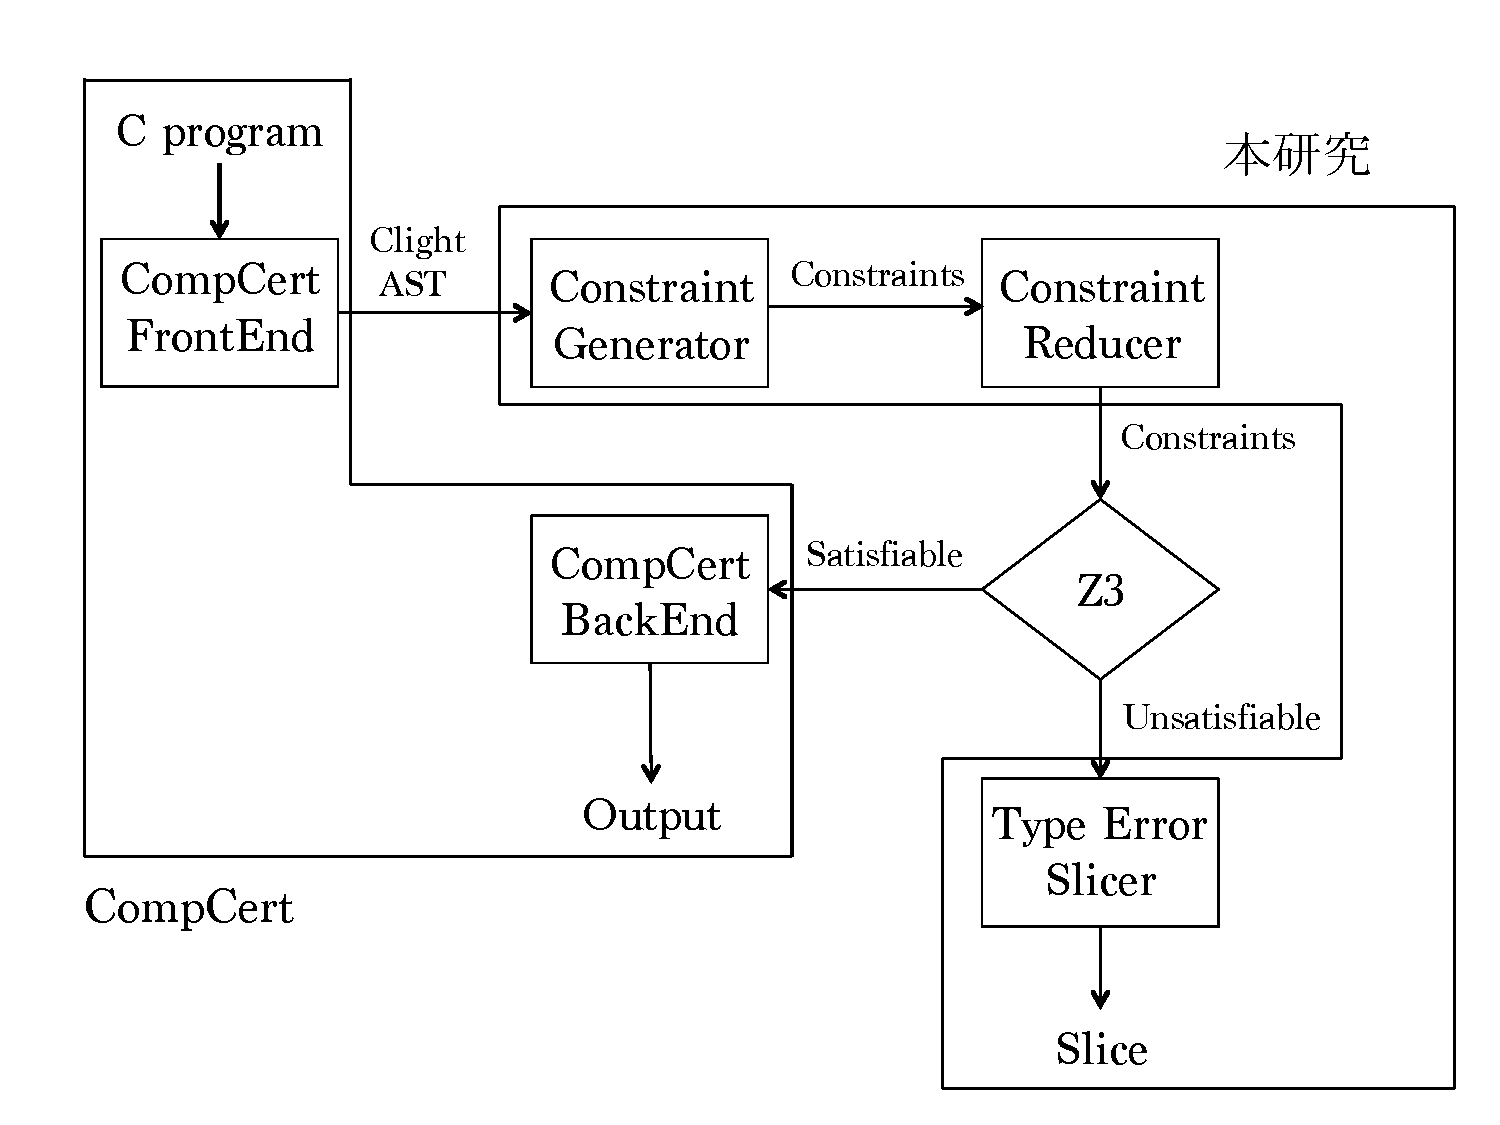
\includegraphics[width=0.9\textwidth]{verifier.pdf}
  \label{impl}
  \caption{実装の全体図}
\end{figure}

CompCertは,C言語のプログラムを受け取るとまず中間言語であるClightに変換す
る.検証器はそのClightの抽象構文木を入力として,型付け規則(図
\ref{typing_stmt})に従い制約式を生成する.そしてその制約式をSMTソルバが解
くことのできる形に変換した後,SMTソルバに渡す.制約式が充足可能であればプ
ログラムに型がつき,メモリ操作に関する誤りが無いことがわかるため,Clihgt
ASTをそのままCompCertに返す.充足不能の場合,SMTソルバはunsat coreを返す.
unsat coreとは,充足不能の原因となっている制約式の部分集合である.型エラー
スライサーは,unsat coreを受け取り,unsat coreに含まれている制約式を生成
した命令の行番号を,スライスとして出力する.


\subsection{制約生成}
この節では,制約生成(Generate)について説明する.まず,扱う制約式につい
て定義する.

\begin{definition}[制約式]
  制約式を図\ref{constr}のように定義する.
\end{definition}
\begin{figure}[htbp]
  \centering
  $
  \begin{aligned}
    c\ (constraints)\ ::=
    \ & \mathtt{Le} (o_{1},\,o_{2},\,loc)\ \\
    |\ &\mathtt{Lt}(o_{1},\,o_{2},\,loc)\ \\
    |\ &\mathtt{Eq}(o_{1},\,o_{2},\,loc)\ \\
    |\ &\mathtt{Empty}(id,\,n,\,loc)\ \\
    |\ &\mathtt{Teq}((id,\,n)\ list,\ (id,\,n)\ list,\ loc)
  \end{aligned}
  $
  \caption{制約式}
  \label{constr}
\end{figure}

各制約式の$loc$は,どの命令から生成された制約式なのかを記録しておくための
情報である.制約式が充足不能となった場合,unsat coreに含まれている制約式
がどの命令から生成されたものなのかを調べ,その命令の行番号を抽出するため
に使用する.

\texttt{Le}は$o_{1} \le o_{2}$,\texttt{Lt}は$o_{1} < o_{2}$,
\texttt{Eq}は$o_{1} = o_{2}$にそれぞれ対応している.\texttt{Empty}は,構
造体の名前を表す$\mathit{id}$,同じ名前でも違う所有権をもつ構造体を区別す
る識別子$n$を受け取る.構造体中の所有権が全て0であるという制約式を表して
いる.\texttt{Teq}は,構造体同士の所有権が等しいという制約式を表している.
各引数がリストになっているのは,型の定義で新しく追加した\texttt{Tplus}を
引数として取れるようにするためである.これにより,構造体を足し算したもの
同士が等しいという制約式も表すことができる.

制約生成の流れは,以下の通りである.入力としてClightプログラムの抽象構文
木を受け取る.図\ref{clight_program}で定義したように,プログラムは関数定
義のリストになっている

\begin{enumerate}
  \item 関数定義から関数環境を生成する
  \item 1の操作を各関数定義に適用する
  \item 引数,局所変数を型環境に追加する
  \item 関数本体に対して所有権に関する制約式を生成する
  \item 3, 4を各関数定義に適用する
\end{enumerate}

まず,関数定義から関数環境を生成する.関数環境は,関数名から関数の型への
写像で定義されている.関数の型\texttt{function}は,引数の型$t_{1}\
\mathit{list}$と,関数実行後の引数の型$t_{2}\ \mathit{list}$,返り値の型
$t$の組で定義されている.返り値の型$t$と引数の型の$t_{1}\ \mathit{list}$
は,関数定義に使われている返り値の型$t$と引数のリスト$\mathit{dcl}_1$をそ
のまま使えば良い.この際,引数の型にポインタ型が含まれている場合,フレッ
シュな所有権変数を割り当てる.また,構造体が含まれている場合も,フレッシュ
な識別子を割り当てる.そして,実行前の引数の型にフレッシュな所有権変数と
構造体にフレッシュな識別子を割り当てたものを関数実行後の引数の型とする.
この操作を各関数定義に対して行う.

\begin{example}[関数環境の生成]
例えば,
\begin{verbatim}
  struct list {
      struct list *next;
      int n
  };

  void free_list(struct list *l)
\end{verbatim}
のように,構造体と関数が定義されている場合,\texttt{free\_list}には,
\begin{verbatim}
function(
  struct(list,
         [(list, comp_ptr(list, 0, Ovar(0)));
          (list, int)]),
  struct(list,
         [(list, comp_ptr(list, 1, Ovar(1)));
         (list, int)]),
  void)
\end{verbatim}
のような型がつく.1引数目の\texttt{Tstruct}が\texttt{free\_list}の引数の
型,2引数目の\texttt{Tstruct}が\texttt{free\_list}を実行した後の引数の型,
3引数目の\texttt{void}が\texttt{free\_list}の返り値の型になっている.この
ように,関数実行後の引数の型は,実行前の引数の型内に含まれる識別子にフレッ
シュなものを割り当てた型にする.そして,(\texttt{free\_list},
\ \texttt{function(...)})を関数環境に追加する.\label{example1}
\end{example}

関数環境の生成後,関数本体について制約式を生成する.まず,関数定義の引数
$\mathit{dcl}_{1}$,局所変数$\mathit{dcl}_{2}$から型環境を生成する.型環
境は,変数名から変数の型への写像で定義されているので,
$\mathit{dcl}_{1},\,\mathit{dcl}_2$をそのまま使えば良い.この際,関数環境
の時と同様に,型内に所有権や構造体の識別子が含まれている場合は,他と被ら
ないように新しい識別子を割り当てる.また,関数本体実行前の局所変数の所有
権は全て0でないといけないという制約式をこの段階で生成する.

この型環境を最初の型環境として,関数本体$s$に対して,図\ref{typing_stmt}
に従い所有権に関する制約式を生成する.基本的には,型付け規則の前提部分を
制約式にしていく.例えば,前提部分の$o = 0$などは,そのまま$\texttt{Eq}(o,\
\texttt{OConst}(0))$とすればよい.

$\texttt{empty}(t)$は,型$t$内の所有権が全て$0$であるということを表してい
る.そこで,型$t$内の所有権が全て$0$であるという制約式を生成する関数
\texttt{empty\_type}を定義する.\texttt{int}や\texttt{float}など,所有権
が割り当てられていない型は,全ての所有権が$0$になっているとみなして良い.
$\texttt{pointer}(t,\ o)$は,$\texttt{Eq}(o,\ \texttt{Oconst}(0))$という
制約式を生成した後,$t$に対して再帰的に\texttt{empty\_type}を適用していく.
$\texttt{struct}(\mathit{id},\ \mathit{fl})$は,$\mathit{fl}$の各要素に対
して\texttt{empty\_type}を適用する.$\texttt{comp\_ptr}(\mathit{id}, n,
o)$は,\texttt{pointer}と同様に$\texttt{Eq}(o,\ \texttt{Oconst}(0))$とい
う制約式を生成した後,参照先に対して所有権が$0$であるという制約式を生成す
る.しかし,\texttt{comp\_ptr}は,再帰を含む構造体内での自己参照をしてい
るポインタのため,\texttt{empty\_type}をそのまま適用していくと,無限ルー
プに陥ってしまう.そこで,図\ref{constr}で定義した$\texttt{Empty}(id, n,
loc)$で,$\texttt{comp\_ptr}$の参照先の所有権が全て$0$である,ということ
を表す.

$t_{1} + t_{2}$は,型$t_1$と型$t_2$を足した型を表している.型同士の足し算
は,所有権同士の足し算として定義されている.そこで,型$t_1$内の所有権と型
$t_2$内の所有権を足す関数\texttt{add\_type}を定義する.基本的には,同じ型
同士しか足し算は行うことができない.所有権が割り当てられていない
\texttt{int}などに関しては,\texttt{empty\_type}と同様に何もせず,そのま
ま$t_{1}$を返す.$\texttt{pointer}(t_{1}',\ o_{1})$と
$\texttt{pointer}(t_{2}',\ o_{2})$に関しては,$t_{1}'$と$t_{2}'$に対して
再帰的に\texttt{add\_type}を適用し,その返り値を$t'$とすると,
$\texttt{pointer}(t',\ \texttt{Oplus}(o_{1},\ o_{2}))$を返す.
\texttt{struct}同士の足し算に関しては,まず構造体の名前が一緒かどうかを確
認する.同じ場合は,フィールドリストの各要素に対して\texttt{add\_type}を
適用する.名前が違う場合は,足し算を行うことはできないので,エラーを返す.
\texttt{comp\_ptr}同士の足し算に関しても,まず同じ構造体内のポインタであ
るかどうかを確認する.また,\texttt{empty\_type}と同様に
\texttt{comp\_ptr}の参照先に関して再帰的に\texttt{add\_type}を実行すると,
無限ループに陥ってしまうため,$\texttt{Tplus}$を使い,\texttt{comp\_ptr}
同士の足し算を表す.

更に,\texttt{comp\_ptr}はポインタ型のため,
$\texttt{comp\_ptr}(\mathit{id},\ n,\ o_{1})$と$\texttt{pointer}(t,\
o_{2})$の足し算を定義することができる.この場合は,\texttt{comp\_ptr}を構
造体を参照しているポインタと読み替える.まず,
$\texttt{comp\_ptr}(\mathit{id},\ n,\ o_{1})$を一回展開する.展開するには,
構造体の名前$\mathit{id}$と構造体内の所有権を区別する識別子$n$を使う.ま
ず$\mathit{id}$と$n$の組で,今までに展開されているかどうかを調べる.展開
されている場合は,以前展開された構造体をそのまま使う.展開されていない場
合,構造体内の\texttt{pointer}と\texttt{comp\_ptr}の所有権と識別子をフレッ
シュなものに書き換えた新たな構造体をつくり,その構造体を参照先にする.こ
の時,$\mathit{id}$と$n$の組が新しく作った構造体を参照しているという情報
を記録しておく.これにより,$\mathit{id}$と$n$の組は常に同じ構造体に展開
されることになる.

$t_{1} = t_{2}$は,型$t_{1}$と型$t_{2}$が等しいという条件を表している.型
同士の等しさは,所有権同士の等しさで定義されている.そこで,型$t_{1}$内の
所有権と型$t_{2}$内の所有権が等しいという制約式を生成する関数
\texttt{eq\_type}を定義する.定義は,\texttt{empty\_type}や
\texttt{add\_type}と同様にすればよい.所有権が割り当てられていない型に関
しては,何もしない.\texttt{pointer}同士に関しては,再帰的に
\texttt{eq\_type}を適用する.\texttt{comp\_ptr}同士に関しては,再帰的に適
用すると無限ループに陥るため,\texttt{Teq}を使い,等しさを表す.
\texttt{comp\_ptr}と\texttt{pointer}に関しては,\texttt{comp\_ptr}を構造
体を参照しているポインタとみなす.\texttt{comp\_ptr}を展開する際の処理も
同様である.

\begin{example}[制約生成]
構造体の定義は例\ref{example1}と同じとする.\\
型環境が
\begin{verbatim}
  l: pointer(struct(list,
                    [(list, comp_ptr(list, 0, Ovar(0)));
                     (list, int)]),
                    Ovar(1))
\end{verbatim}
のもとで,
\begin{verbatim}
  free(l)
\end{verbatim}
を実行すると,実行後の型環境が
\begin{verbatim}
  l: pointer(struct(list,
                    [(list, comp_ptr(list, 0, Ovar(0)));
                     (list, int)])struct(list,
                    [(list, comp_ptr(list, 0, Ovar(0)));
                     (list, int)]),
                    Ovar(2))
\end{verbatim}
になり,制約式として
\begin{verbatim}
  Eq(Ovar(1), Oconst(1), loc);
  empty_type(struct(list,
                    [(list, comp_ptr(list, 0, Ovar(0)));
                     (list, int)]));
  Eq(Ovar(2), Oconst(0), loc);
\end{verbatim}
が生成される.更に\texttt{empty\_type}からは,
\begin{verbatim}
  Eq(Ovar(0), Oconst(0), loc);
  Empty(list, 0, loc);
\end{verbatim}
が生成される.
\texttt{loc}には,\texttt{free(l)}のプログラム中での行番号が入る.
\end{example}

関数本体に対して制約式の生成が終わると,関数本体実行後の型環境が得られる.
この型環境内に含まれる引数の型は,関数環境内に追加されている関数実行後の
引数の型と一致しなければならない.また,関数本体実行後には関数の局所変数
の所有権は全て0になっていなければならない.この2つの条件に関しても制約式
を生成する.この操作を各関数定義に対して適用する.

以上の操作によって得られた制約式を集めたものが制約式の集合となる.この制
約式の集合をSMTソルバで解く.\texttt{Le},\texttt{Lt},\texttt{Eq}は不等
式の形をしているため,そのままSMTソルバで解くことができるが,
\texttt{Empty},\texttt{Teq}はこのままではSMTソルバは解くことができない.
そのため,SMTソルバに解ける形に変換する必要がある.

\subsection{制約式変換}
この節では,前節で生成した制約式をSMTソルバに解ける形に変換する手法につい
て述べる.制約式\texttt{Empty}と\texttt{Teq}はそのままではSMTソルバは解く
ことができないため,不等式の形まで変換する必要がある.制約式の変換は,
前処理と実際に変換する段階にわけられる.

再帰のある構造体に関する制約式は前節で述べたように,ポインタ型と同様に再
帰的に展開して生成するという方法で生成すると,無限に展開されてしまう.そ
のため,どこかで展開をとめる必要がある.先行研究では,テンプレート型
$(\mu\alpha.\ \texttt{ref}_{f1})\ \texttt{ref}_{f0}$を使用して,展開回数
を制限していた.この型は,ある展開回数までは別々の所有権が割り当てられて
いるが,それ以降は同じ所有権が割り当てられているとみなすという近似をして
いることになる.しかし,先行研究で実装された検証器では,十分に多い回数展
開を行って制約式を生成するだけで,それ以降は同じ所有権が割り当てられてい
るという部分は実装していなかった.

本研究では,前処理の段階でプログラム中で何回か展開した先のメモリ領域に対
して操作を行っている場合,その回数分は展開を行う.そして,変換する段階で
それ以降に関しては同じ所有権が割り当てられているとみなすという処理を行う.
これにより,より理論に基づいた実装になっている.


\subsubsection{前処理}
前処理の段階では,制約生成の段階で既に展開されたことのある
\texttt{comp\_ptr}を展開する.制約生成の,\texttt{add\_type}や
\texttt{eq\_type}内で,$\texttt{comp\_ptr}(\mathit{id},\ n,\ o)$と
$\texttt{pointer}(t,\ o)$との間の足し算や型の等しさなどを求めると,
$\texttt{comp\_ptr}(\mathit{id},\ n,\ o)$は一回展開され,$\mathit{id}$と
$n$の組がどの構造体に展開されるかという情報は記録される.\texttt{Empty}や
\texttt{Teq}内の$\mathit{id}$と$n$の組が制約生成の段階で記録されているか
どうかを調べ,記録されている場合は展開先の構造体の
$\texttt{comp\_ptr}(\mathit{id},\ n',\ o')$を使い,書き換えるということを
行う.この操作を$\mathit{id}$と$n'$の組に関しても再帰的に適用していくこと
で,制約生成の段階で展開された回数分,つまりプログラム中で展開された回数
分は,構造体を展開するというということを実現している.

\begin{example}[前処理: Empty]
  構造体の定義は例\ref{example1}と同じである.
  制約式
\begin{verbatim}
    Empty(list, 1, loc);
\end{verbatim}
  が生成され,制約生成の段階で,
\begin{verbatim}
    (list, 1) -> struct(list,
                        [(list, comp_ptr(list, 2, Ovar(2)));
                         (list, int)])
    (list, 2) -> struct(list
                        [(list, comp_ptr(list, 3, Ovar(3)));
                         (list, int)])
\end{verbatim}
  という情報が記録されていた場合,前処理によって制約式は
\begin{verbatim}
    Empty(list, 3, loc);
    Eq(Ovar(2), Oconst(0), loc);
    Eq(Ovar(3), Oconst(0), loc);
\end{verbatim}
  という制約式に書き換えられる.
\end{example}

\texttt{Teq}の場合も同様に展開を行うのだが,\texttt{Teq}の引数はリストに
なっているため,複数の$\mathit{id}$と$n$の組が出現することがある.この場
合は,リスト内の全ての$\mathit{id}$と$n$の組が制約生成の段階で,展開され
ている場合のみ書き換えを行い,リスト内の要素の一部だけ記録されている場合
は展開を行わない.


\subsubsection{制約の不等式への変換}
前処理の段階で,制約生成の段階で記録された$\mathit{id}$と$n$の情報を使っ
て構造体を展開し制約式を書き換えたため,変換の段階では記録されていない
$\mathit{id}$と$n$に関しての処理を行う.

具体的には,前処理が終わった段階で記録されていない$\mathit{id}$と$n$の組
は全て,自分自身と同じ型の構造体を参照しているとみなす.そしてその情報を
使い,前処理と同様に制約式を書き換えていく.制約式が書き換え前と書き換え
後とで変化しなくなった時点で,書き換えをやめる.この操作が終わると,
\texttt{Empty}と\texttt{Teq}からは新しい制約式が生成されることはないため,
制約式から\texttt{Empty}と\texttt{Teq}を消去してもよい.消去後の制約式に
は,\texttt{Lt},\texttt{Le},\texttt{Eq}しか入っていないため,SMTソルバ
で解ける形になっている.

\begin{example}[変換: Teq]
  構造体の定義は例\ref{example1}と同じである.
  制約式
\begin{verbatim}
    Teq([(list, 1)], [(list, 2); (list, 3)])
\end{verbatim}
  が生成され,前処理の段階で
\begin{verbatim}
    (list, 1) -> struct(list,
                        [(list, comp_ptr(list, 4, Ovar(4)));
                         (list, int)])
\end{verbatim}
  という情報が記録されてい場合,\verb|(list, 2)|と\verb|(list, 3)|に関し
  て情報が記録されていないため,前処理の段階ではこの制約式の書き換えは行
  われない.変換の段階では,まず\verb|(list, 2)|と\verb|(list, 3)|に関し
  て自分自身を参照しているという情報を追加する.
\begin{verbatim}
    (list, 1) -> struct(list,
                        [(list, comp_ptr(list, 4, Ovar(4)));
                         (list, int)])
    (list, 2) -> struct(list,
                        [(list, comp_ptr(list, 2, Ovar(5)));
                         (list, int)])
    (list, 3) -> struct(list,
                        [(list, comp_ptr(list, 3, Ovar(6)));
                         (list, int)])
    (list, 4) -> struct(list,
                        [(list, comp_ptr(list, 4, Ovar(4)));
                         (list, int)])
\end{verbatim}
  この情報を使い制約式を書き換えると
\begin{verbatim}
    Teq([(list, 4)], [(list, 2); (list, 3)]);
    Eq(Ovar(4), Oplus(Ovar(5), Ovar(6)));
\end{verbatim}
  になる.そして,\texttt{Teq}からはもう新しい制約式は生成されないため
  \texttt{Teq}は消去され,
\begin{verbatim}
    Eq(Ovar(4), Oplus(Ovar(5), Ovar(6)));
\end{verbatim}
  だけになる.
\end{example}
\subsection{制約解消}
制約式変換を終えた制約式は,SMTソルバで解ける形になっている.その制約式を
SMTソルバで解くことで,制約式が充足可能かどうか判定することができる.今回
の実装ではSMTソルバには,Z3 \cite{DBLP:conf/tacas/MouraB08}を使用した.ソ
ルバが制約を充足可能と判定した場合は,プログラムに型がつき,メモリ操作に
関する誤りが発生していないことがわかる.ソルバが充足不能と判定した場合は,
同時にunsat coreを返す.unsat coreとは,制約式の充足不能性の原因となって
いる制約式の部分集合である.unsatの場合は,プログラム中のどこかでメモリ操
作に関する誤りがあり,その箇所が型エラーの原因となっている.その箇所を特
定するのは,小さなプログラムでは容易だが,大きなプログラムだと困難である.
そこで,unsat coreを用いて型エラーの原因となっている命令の集合をプログラ
ム中から切り出して,表示する.この情報は,プログラマが型エラーの原因を特
定するのに役立つと考えられる.

\subsection{型エラースライサー}
型エラースライサーは,制約式の集合とunsat coreを入力として,型エラーの原
因に関係している命令の行番号をスライスとして出力する.unsat coreには制約
式の充足不能性の原因,つまり型エラーの原因となっている制約式が含まれてい
る.そこで,unsat coreに含まれている各制約式がそれぞれどの命令から生成さ
れたものなのかを調べる.制約式には,その制約式を生成した命令の行番号
$loc$が含まれているので,unsat coreに含まれている各制約式の$loc$をまとめ
たものをスライスとすればよい.

今回ソルバとして使用したZ3は,unsat coreを制約式の名前で返す.そのため,
Z3に制約式を渡す際に,各制約式に名前をつけ,どの制約式にどういう名前をつ
けたのかを記録しておくことで,Z3がunsat coreとして返してきた制約式の名前
から制約式を特定し,$loc$を調べることができる.

\begin{example}[型エラースライサー]
  プログラム \ref{rec_struct_unsat}\ (付録参照)\ を例に挙げる.このプログラム
  は,再帰を含む構造体\texttt{list}を使って単方向リストの操作を行っている
  プログラムである.\texttt{make\_list}で単方向リストの各要素に新しいメモ
  リ領域を割り当て,\texttt{free\_all\_list}でそれら全てを解放する.しか
  し,\texttt{free\_all\_list}内で,\texttt{free}を実行し忘れているため,
  メモリリークが発生している.

  このプログラムから制約式を生成し,Z3で解くと
\begin{verbatim}
    unsat
    (c_70 c_67 c_66 c_64 c_54 c_52
     c_49 c_48 c_32 c_31 c_8 c_3 c_7)
\end{verbatim}
  を返す.メモリリークが発生しているため制約式は充足不能である.
  また充足不能のため,unsat coreを一緒に返している.
  unsat coreの各要素は,制約式の名前である.
  型エラースライサーは,これらの名前がついた制約式を生成した命令を探し
  それの行番号をスライスとして出力する.
\begin{verbatim}
    [11; 18; 30; 32; 39; 40; 43]
\end{verbatim}

  $30$行目の\texttt{malloc}で新しいメモリ領域を
  割当て,$32$行目の\texttt{return}でその変数を返り値としているため,$39$行
  目で\texttt{make\_list}を呼び出しその返り値を代入している変数\texttt{l}に
  は,所有権が与えられているはずである.しかし,$40$行目で
  \texttt{free\_all\_list}を呼び出しているにもかかわらず,$43$行目で,関数
  の終了時には関数の局所変数の所有権,つまり\texttt{l}内の所有権は全て$0$に
  なっていないといけないという条件をみたすことができていない.更に$18$行目
  の\texttt{free\_all\_list}もスライスに含まれていることから,
  \texttt{free\_all\_list}の実装が間違っているのではないかと,プログラマは
  推測することができる.
\end{example}

\section{予備実験}
\label{section5}
この章では,本研究で実装した検証器に対して行った予備実験について述べる.

\begin{table}[htbp]
  \footnotesize
  \centering
  \caption{実験結果}
  \label{ex_table}
  \begin{tabular}[tb]{|l|r|r|r|r|r|r|}
    \hline
    Program & LOC & Time\_g & SIZE\_g & Time\_r & SIZE\_r & Time\_s \\ \hline\hline
    \verb|sl_app| & 55 & 0.165 & 200 & 0.748 & 193 &  34.0 \\ \hline
    \verb|sl_free| & 44 & 0.112 & 114 & 0.505 & 110 & 26.5 \\ \hline
    \verb|sl_merge| & 60 & 0.280 & 250 & 1.395 & 237 & 37.5 \\ \hline
    \verb|sl_mut| & 60 & 0.140 & 149 & 0.495 & 145 & 30.9 \\ \hline
    \verb|sl_reverse| & 63 & 0.173 & 222 & 0.901 & 205 & 33.2 \\ \hline
    \verb|sl_search| & 60 & 0.189 & 189 & 0.654 & 176 & 36.8 \\ \hline
  \end{tabular}
\end{table}

表\ref{ex_table}は実験結果をまとめたものである.
各列の意味は以下のとおりである.
\begin{itemize}
  \item LOC: プログラムの行数
  \item Time\_g: 制約生成にかかった時間(msec)
  \item SIZE\_g: 生成された制約式の数
  \item Time\_r: 制約変換にかかった時間(msec)
  \item SIZE\_g: 変換後の制約式の数
  \item Time\_s: 制約解消にかかった時間(msec)
\end{itemize}

実験に用いた計算環境は CPU: Intel Core i7 1.7 GHz,MEM:8GB,OS:OSX
10.9.5 である.使用したソフトの各バージョンは,CompCert: 2.4, OCaml:
4.02.1, Z3: 4.3.2 である.

いずれのプログラムも,単方向リストを操作するプログラムで,末永らが先行研
究で実装した検証器に対して行った予備実験で使われたプログラムと同等のもの
である.各プログラムには,$\texttt{assert\_null}(p)$という注釈を手動で適
当な箇所に挿入してある.これは,\ref{section3}で述べたように,ポインタの
参照先を\texttt{null}とみなして,任意の型をもてるようにするための命令であ
る.

\verb|sl_app|は,リストを2つ生成した後,片方のリストをもう片方のリストの
最後尾に繋げたリストを生成し,それを繋げたリストを生成し,そのリストを解
放する.\verb|sl_free|は,単純にリストを生成しそれを解放する.
\verb|sl_merge|は,リストを2つ生成した後,それらのリストの先頭から要素を
ランダムに選んで繋げたリストを生成し,そのリストを解放する.
\verb|sl_mut|は,\verb|sl_free|と同じ操作を行っているが,相互再帰関数を使っ
て解放を行っている.\verb|sl_reverse|は,リストを生成した後,そのリストの
順番を逆にし,そのリストを解放する.\verb|sl_search|は,リストを生成した
後,リストから要素を一つ取り出してその要素を除いたリストを生成し,取り出
した要素とそれを除いたリストを解放する.

いずれのプログラムもサイズは大きくないが,非常に高速に検出することができ
ている.生成された制約式が変換によって数が減っているのは,変換の際に生成
された制約式の中に,同じ制約式があるとそれを消す操作を行っているためであ
る.

また,各プログラムに対してメモリリークが発生するように,\texttt{free}命
令を消すなどの書き換えを行い,実験を行った.結果として,全てのプログラムに対
して検証器は充足不能と判定し,エラーを正しく検出していることを確認した.

\section{関連研究}
\label{section6}
本研究では,末永らが提案したメモリリークを静的に検出する型システム
\cite{DBLP:conf/aplas/SuenagaK09}を制御文で拡張しした.また,その拡張した
型システムに基いて検証器を実装した.検証器の実装においては,Leoryらによっ
て実装されたC言語のコンパイラCompCert
\cite{DBLP:journals/cacm/Leroy09,DBLP:conf/itp/KrebbersLW14 }を拡張する形
で実装した.また型システムの拡張も,CompCertで使われている中間言語
Clight \cite{DBLP:journals/jar/BlazyL09} を元にしている.

CompCertを使用した他の研究としては\cite{DBLP:conf/popl/StewartBCA15}など
がある.従来のCompCertは他のモジュール内の関数の呼び出しの正しさはは保証
しない.そこで,この研究は他のモジュール内の関数の呼び出しなどの正しさも
保証するComposite CompCertを提案している.

本研究で,SMTソルバとして使用した Z3 を利用した研究として
\cite{DBLP:conf/fmcad/McMillan11}などがある.これは,Z3を利用して,モデル
検査の分野で使用される補間を求める手法を提案している.

型エラースライサーは,静的型付けの行われている関数型言語に対して,型エラー
が発生した際に,型エラーに関係しているプログラム地点をスライスとして出力
するツールである\cite{DBLP:conf/esop/HaackW03,DBLP:conf/dsl/DineshT97}.
更に,型エラースライサーは本来,関数型言語を対象としていたが,近年Javaな
どの言語に対しても研究が行われている\cite{DBLP:conf/pepm/BoustaniH09}.一
般の静的型付け言語において,型推論はプログラムを抽象構文木に変換した後,
各ノードに対して型付け規則に基いて型がつくかどうか確認していき,失敗した
場合,失敗したノードを1つだけ型エラーの原因として出力する.しかし,型エラー
の原因が1つしか挙げられないため,プログラマは型エラーの原因を正確に特定す
ることができない.そこで型エラースライサーは,各ノードから生成された制約
式にラベルをつけ,制約式全体が充足不能とわかった場合,充足不能となってい
る最小の制約式の集合を抽出し,その集合に含まれている制約式のラベルからプ
ログラム地点を特定し,スライスとして出力するということをしている.本研究
の型エラースライサーもこの考えに基づいて実装をしている.\ref{section4}で
述べたように,制約式の充足不能の原因を抽出する際に,SMTソルバが返す
unsat core を用いている.また,これまでの型エラースライサーは単純型を対象
としていたが,本研究では,所有権型を対象としている.\cite{飯村枝里2007,
飯村枝里2008}では,並行プログラミングにおけるレースの原因やデッドロックの
原因を型エラースライサーを用いて特定しているが,制約式の充足不能の原因特
定に unsat core は用いられていない.

他のメモリリークの検証器は,XieらによるSATソルバを用いた
\cite{DBLP:conf/sigsoft/XieA05}や,Cheremらによるグラフを用いた
\cite{DBLP:conf/pldi/CheremPR07}などがある.しかし,両方ともループを健全
な形で扱うことができない.

Hoare 論理を拡張して,領域の確保や解放,領域へのアクセスなどメモリに関す
る操作をを扱えるようにした体系としてSeparation Logic
\cite{DBLP:conf/lics/Reynolds02}が提案されている.この Separation Logic
に基いて,メモリリークの検出やエイリアス解析などを行う手法として Shape
analysis
\cite{DBLP:conf/cav/BerdineCCDOWY07,DBLP:conf/tacas/DistefanoOY06,
DBLP:conf/pldi/GuoVA07} という手法がある.しかし,これらの手法は検出に非
常に時間がかってしまう.

\section{おわりに}
\label{section7}
本研究では,末永らが提案したメモリリークを静的に検出するための型システム
を制御文で拡張し,その拡張した型システムに基いて検証器を実装することで,
検証器の信頼度を高めた.また,型エラースライサーを組み込むことで,検証器
の利便性も高めた.更に,予備実験を行いいくつかのプログラムに対して,メモ
リリークを正しく検出できることを確かめた.

今後の課題として,まず扱える構文を増やすことが挙げられる.\ref{section3}
で述べたように,配列型,キャストやアドレス演算子などの式,\texttt{goto}や
\texttt{label}などの文,大域変数は,本研究で拡張した型システムではまだ扱っ
ていない.\texttt{goto}や\texttt{label}などは,\texttt{break}や
\texttt{continue}の考えを応用すれば扱えるようになると考えられる.また,拡
張した型システムの健全性の証明を行っていない.元の型システムでは,プログ
ラムに型がつけば,プログラム中でメモリリークが起きてないことが保証されて
いたが,今回拡張した制御文などの構文に関しては,その性質の証明ができてい
ない.更に,より大きなプログラムに対して実験を行うことが挙げられる.今回
の予備実験ではいずれも小さなプログラムに対してのみ実験を行ったので,より
大きなプログラムでもメモリリークを正しく検出できるか,どの程度早く検出で
きるかなどを確かめる必要がある.同時に,型エラースライサーが型エラーの原
因の特定にどの程度有効なのかを確認し,改良していく必要がある.

\acknowledgments

はじめに,本研究に際し,テーマの決定から,検証器の実装,本論文の執筆に至
るまで,日頃から多大なる御指導を賜りました末永幸平准教授に深く感謝致しま
す.また,本研究に有益なご助言を下さいました五十嵐淳教授,馬谷誠二助教
に御礼を申し上げます.更に,内見を引き受けてくださり,本研究にコメントを
下さいました高瀬英希助教に感謝申し上げます.最後に,日頃の雑談に付き合っ
てもらうだけでなく,本研究に様々な指摘まで下さった五十嵐・末永研究室の皆
様に感謝致します.



\bibliographystyle{kuisunsrt}
\bibliography{thesis}

\appendix
\section{プログラム例}
\begin{lstlisting}[caption={再帰を含む構造体},label={rec_struct_unsat}]
struct list{
    struct list *next;
    int e;
};

struct list *malloc(unsigned int size);
void free(void*);
void assert_null(void*);

void free_all_list (struct list *l) {
    struct list *p;

    if (l == '\0') {
        assert_null(l);
        return;
    } else {
        p = l->next;
        free_all_list(p);
        // free(l);
    }
}

struct list *make_list(unsigned int n) {
    struct list *ret;

    if (n == 0) {
        assert_null (ret);
        return ret;
    } else {
        ret = malloc(sizeof (struct list));
        ret->next = make_list(n-1);
        return ret;
    }
}

int main() {
    struct list *l;

    l = make_list(3);
    free_all_list(l);

    return 0;
}

\end{lstlisting}

\end{document}